\documentclass[aps, prb, floatfix, twocolumn, notitlepage, superscriptaddress, 10pt]{revtex4-2}
\usepackage{xcolor}
\usepackage{amsmath, amsthm, amssymb, bbold}
%\usepackage{float}
\usepackage[normalem]{ulem}
\usepackage{cancel}
\usepackage{bm}
\usepackage{microtype}
\usepackage{hyperref}
\usepackage{setspace}
\hypersetup{colorlinks,linkcolor=blue,urlcolor=blue,citecolor=blue}
%\usepackage[magyar]{babel}
%\usepackage[makeroom]{cancel}
\usepackage{amsmath}    % need for subequations
\usepackage{amssymb}
\usepackage{graphicx}   % need for figures
\usepackage{verbatim}   % useful for program listings
\usepackage{color}      % use if color is used in text
%\usepackage{subfigure}  % use for side-by-side figures
\usepackage{hyperref}   % use for hypertext links, including those to external documents and URLs
%\usepackage{blindtext}
\usepackage[normalem]{ulem}
%\usepackage{xpatch}
\usepackage{natbib}
\usepackage{fixmath}
\usepackage{enumitem}
\usepackage{dsfont}

\def \brc #1{\left\lbrace #1 \right\rbrace}
\def \loc {\mathrm{loc}}
%\def \ttau {{\tilde \tau}}
\def \ttau {{\tau}}
% Until we finalize the notation of the total particle number

\newcommand{\n}{N}
\hypersetup{colorlinks,linkcolor=blue,urlcolor=blue,citecolor=blue}
\newcommand{\uv}[1]{\ensuremath{\mathbf{\hat{#1}}}} % for unit vector
\newcommand{\gv}[1]{\ensuremath{\mbox{\boldmath$ #1 $}}} % 
\newcommand{\rem}[1]{  {\color{red} #1}  }
%\newcommand{\g}[1]{{\bf #1 }}
\newcommand{\beq}{\begin{equation}}
\newcommand{\eeq}{\end{equation}}
\newcommand{\bea}{\begin{eqnarray}}
\newcommand{\eea}{\end{eqnarray}}
\newcommand{\blabel}{\,b}
\newcommand{\alabel}{\,a}
\newcommand{\Lspace}{{\mathit{\mathbb{L}}}}
\newcommand{\g}[1]{{\color{blue}#1}}
\newcommand{\red}{\color{red}}
\newcommand{\dom}[1]{\color{purple} @Dominik: #1}

\newcommand{\bbGamma}{{\mathpalette\makebbGamma\relax}}
\newcommand{\makebbGamma}[2]{%
  \raisebox{\depth}{\scalebox{1}[-1]{$\mathsurround=0pt#1\mathbb{L}$}}%
}

\newcommand{\e}{\text e}
\newcommand{\zp}{\mathbb Z^+}
\newcommand{\z}{\mathbb Z}
\newcommand{\hint}{H_{\text{int}}}
\newcommand{\re}{\text{Re }}
\newcommand{\hc}{\text{h.c.}}
\newcommand{\cc}{\text{c.c.}}
\newcommand{\w}{\omega}
\newcommand{\be}{\begin{equation}}
\newcommand{\ee}{\end{equation}}
\newcommand{\Nedge}{N_{\rm edge}}



\definecolor{darkgreen}{rgb}{0,0.5,0}
\definecolor{orange}{rgb}{1,0.5,0}
\definecolor{grey}{rgb}{.6,.6,.6}
\newcommand{\rc}[1]{\textcolor{red}{#1}}
%\bibliographystyle{apsrev4-1}
%\newcommand{\jav}[1]{#1}
\newcommand{\scrap}[1]{{\color{orange}{\sout{#1}}}}
\newcommand{\cpm}[1]{{\color{blue}{#1}}}

\newcommand{\dr}{\text d^3r}
\newcommand{\dfi}{\text d\varphi}
\newcommand{\dd}{\text d}
\newcommand{\tr}{\tilde r}
\newcommand{\tn}{\tilde n}
\newcommand{\tz}{\tilde z}
\newcommand{\tc}{\tilde c}
\newcommand{\tS}{\tilde S}
\newcommand{\tT}{T}

\newcommand{\heff}{H_{\text{eff}}}
\newcommand{\hkin}{H_{\text{kin}}}

\newcommand{\pp}{P^{++}+P^{--}}
\newcommand{\ps}{P^{\text(S)}}
\newcommand{\pa}{P^{\text(A)}}
\newcommand{\psn}{P_{S=0}}
\newcommand{\pse}{P_{S=1}}
\newcommand{\eppn}{E^{+}_{0}}
\newcommand{\eppe}{E^{+}_{1}}
\newcommand{\ese}{E^{\text{(S)}}_{1}}
\newcommand{\esn}{E^{\text{(S)}}_{0}}
\newcommand{\eae}{E^{\text{(A)}}_{1}}
\newcommand{\ean}{E^{\text{(A)}}_{0}}
\newcommand{\kent}{k\in\text{NT}}
\newcommand{\meV}{\,{\rm meV}}
\newcommand{\ie}{{\it i.e. }}
\newcommand{\bra}[1]{\langle #1|}
\newcommand{\ket}[1]{|#1\rangle}
\newcommand{\average}[1]{\langle #1\rangle}

%\newcommand{\scrap}[1]{{\color{red}{\sout{#1}}}}


\newcommand{\bK}{\mathbf K}
\newcommand{\bS}{\mathbf S}
\newcommand{\bk}{\mathbf k}
\newcommand{\bq}{\mathbf q}
\newcommand{\ba}{\mathbf a}
\newcommand{\bC}{\mathbf C}
\newcommand{\bJ}{\mathbf J}
\newcommand{\bH}{\mathbf H}
\newcommand{\bchi}{\boldsymbol \chi}
\newcommand{\bkappa}{\boldsymbol \kappa}
\newcommand{\bx}{\mathbf x}
\newcommand{\br}{\mathbf r}
\newcommand{\brp}{{\mathbf r}'}
\newcommand{\bxp}{{\mathbf x}'}


%\newcommand{\g}{{\gamma}}
\newcommand{\ds}{\displaystyle}
\newcommand{\1}{{1\hspace*{-0.5ex} \textrm{l} \hspace*{0.5ex}}}

\newcommand{\cL}{{\cal L }}
\newcommand{\fL}{\mathfrak{ L }}
\newcommand{\cH}{{\cal H }}
\newcommand{\fH}{\mathfrak{H }}

\newcommand{\cQ}{{\cal Q}}
\newcommand{\cD}{{\cal D}}
\newcommand{\cG}{{\cal G}}
\newcommand{\cg}{{\cal g}}
\newcommand{\cS}{{\cal S}}
\newcommand{\cJ}{{\cal J}}
\newcommand{\cN}{{\cal N}}
\newcommand{\chU}{\hat{\cal U}}
\newcommand{\hU}{{\hat U}}

\newcommand{\ketL}[1]{|#1 )}
\newcommand{\braL}[1]{( #1|}
\newcommand{\averageL}[1]{( #1 )}
\newcommand{\tsigma}{{\tilde \sigma}}

\def\doubleunderline#1{\underline{\underline{#1}}}

\newcommand{\mk}[1]{{\color{blue} #1}}


\newcommand{\tp}[1]{{\color{darkgreen} #1}}

\begin{document}
\title{Collective Wigner crystal tunneling in carbon nanotubes}
\author{Dominik  Szombathy}
\affiliation{Department of Theoretical Physics,  Institute of Physics, Budapest University of Technology and Economics,  Budafoki \'ut 8., H-1111 Budapest, Hungary}
\affiliation{MTA-BME Quantum Dynamics and Correlations Research Group, 
Institute of Physics, Budapest University of Technology and Economics,  Budafoki \'ut 8., H-1111 Budapest, Hungary}
\affiliation{Nokia Bell Labs, Nokia Solutions and Networks Kft, 1083 Budapest, B\'okay J\'anos u. 36-42, Hungary}
\author{Mikl\'os Antal Werner}
\affiliation{MTA-BME Quantum Dynamics and Correlations Research Group, 
Institute of Physics, Budapest University of Technology and Economics,  Budafoki \'ut 8., H-1111 Budapest, Hungary}
\affiliation{Strongly Correlated Systems 'Lend\" ulet' Research Group, 
Wigner Research Centre for Physics, P.O. Box 49, 1525 Budapest, Hungary}
\author{C\u at\u alin Pa\c scu Moca}
\affiliation{MTA-BME Quantum Dynamics and Correlations Research Group, Budapest University of Technology and Economics, M\"uegyetem rkp. 3., H-1111 Budapest, Hungary }
\affiliation{Department of Physics, University of Oradea,  410087, Oradea, Romania}
\author{\"Ors Legeza}
\affiliation{Strongly Correlated Systems 'Lend\" ulet' Research Group, 
Wigner Research Centre for Physics, P.O. Box 49, 1525 Budapest, Hungary}
\affiliation{Institute for Advanced Study,Technical University of Munich, Lichtenbergstrasse 2a, 85748 Garching, Germany}
\author{Assaf Hamo}
\affiliation{Department of Physics, Harvard University, Cambridge, MA 02138, USA}
\author{Shahal  Ilani}
\affiliation{Department of Condensed Matter Physics, Weizmann Institute of Science, Rehovot 76100, Israel.}
\author{Gergely Zar\'and}
\affiliation{MTA-BME Quantum Dynamics and Correlations Research Group, Budapest University of Technology and Economics, M\"uegyetem rkp. 3., H-1111 Budapest, Hungary }
\date{\today}
\begin{abstract}
The collective tunneling of  a a Wigner necklace –  a crystalline state of a small number of strongly interacting 
electrons  confined to  a suspended nanotube and subject to a double well potential –  is theoretically analyzed and compared with experiments 
in  [Shapir \emph{et al.}, Science {\bf 364}, 870 (2019)]. Density Matrix Renormalization Group 
computations, exact diagonalization, and instanton theory provide a consistent description of this very strongly interacting 
system, and show good agreement with experiments.  Experimentally  extracted and  theoretically computed tunneling amplitudes 
exhibit a scaling collapse. Collective quantum fluctuations renormalize the tunneling, and substantially enhance it  as 
the number of electrons  increases.
\end{abstract}
\maketitle

\section{Introduction}

%Carbon nanotubes (CN) have opened up a wide range of possibilities for developing new devices with unique electronic, mechanical, and 
%physical properties since their discovery~\cite{Salvetat.1999, KouwenhovenRMP, Ayala.2010, PANTANO2004789}.
%They come into a multitude of geometries, as single wall or multiple wall CNs~\cite{Charlier.2007,Kukovecz2013} and can exibit metallic and semiconducting
%behavior depending on their diameter and chirality~\cite{Krupke.2003}. 
%The electronic and mechanical properties of CN can be modified by controlling 
%their diameter, chirality, length, or doping level, making them a versatile platform for tunable ballistic or diffusive quantum wires~\cite{Frank.1998, Bandow.1998} or in the field of nanoelectronics~\cite{TSUKAGOSHI2002107}.
%Additionally, the one-dimensional nature of CNs makes them attractive for  
%exploring novel physical phenomena, such as one dimensional quantum dots~\cite{Tans.1997,Bockrath.1997}, 
%proximity induced superconductivity~\cite{Kasumov.1999,Morpurgo.1999}, for demonstrating the universality of the 
%Kondo effect~\cite{Nygard.2000}, the emergence of Luttinger liquid behavior~\cite{Bockrath.1999,Levitov.2003}
%or the formation of the Wigner crystal~\cite{Deshpande.2008,Pecker.2013, Shapir.2019}. 

While investigating correlation effects in electron liquids, Eugene Wigner conjectured in 1934 the existence of an electron crystal~\cite{Wigner1934}, today referred to as the \emph{Wigner crystal}. In his seminal work, 
Wigner noticed that  the interaction energy of a three-dimensional electron gas  
scales as $E_{\text{int}}\sim n^{1/3}$ with their density $n$, and dominates over the kinetic energy $E_K\sim n^{2/3}$
in the very dilute limit. 
Therefore,  electrons must become localized at very small carrier concentrations, and form a crystal. 
The kinetic energy of the electrons increases upon compression,  and the crystal  melts due to quantum 
and thermal fluctuations into an electron liquid. 
A similar solid–liquid (quantum) phase transition occurs in two spatial dimensions. In one dimension, however, 
quantum fluctuations always destroy long-range order, and no phase transition takes place: 
only a cross-over  between a Luttinger liquid-like  and a dilute regime with power-law crystalline correlations
appears~\cite{Schulz1993}.  

Since the predictions of Wigner, tremendous effort has been devoted to detect and understand this quantum crystal. 
While  these efforts remained unsuccessful in three dimensions, Wigner crystal phases and correlations 
have been demonstrated   in two-dimensional structures~
\cite{Andrei1988, Meyer2009, Jiang1990, Goldman1990, Buhmann1991,Santos1992, Shirahama1995,Yoon1999,Chen2006,Zhu2010, Tiemann2014,Deng2016, Deng2019, Ma2020, Regan2020, Smoleski2021,Zhou2021,Li2021, Villegas2021, Falson2022, Hossain2022} as well as  more recently  in one 
dimension~\cite{Shapir.2019,Deshpande.2008}. 

%The formation of a Wigner crystal in suspended nanotubes was first observed indirectly in Ref.~\cite{Deshpande.2008} through magnetic field measurements as a function of carrier density, measurements which  could be explained using a Wigner crystal model. Later, a Wigner molecule was reported in nanotubes in which two electrons were localized in two separate sides of an ultraclean nanotube, and the spatial structure was extracted from  the energy spectrum~\cite{Pecker.2013}. Recently, the real space structure of the Wigner crystal was directly observed for the first time by imaging the charge density~\cite{Shapir.2019}, providing an unambiguous fingerprint for the real-space formation of the Wigner crystal. Additionally, to probe the quantum nature of the Wigner crystal, the correlations between electrons were measured by creating a tunneling barrier that causes the electrons to tunnel collectively.
In particular, in Ref.~\cite{Shapir.2019} the real space structure of a small one-dimensional crystal in a carbon nanotube 
has been carefully probed, and the \emph{collective tunneling} of the crystal observed. In this work, we focus on this latter 
phenomenon, and model and analyze the tunneling of a small, one-dimensional Wigner crystal. 

The  set-up of Ref.~\cite{Shapir.2019} is displayed in Fig.\ref{fig:experimental_setup}(a).
A carbon nanotube is suspended and gated appropriately. Gates on the r.h.s., underneath the nanotube
are used to trap $N$ electrons (or holes), and  to create a confining potential $V(z)$ at wish, with $z$ 
the electrons' coordinate along the nanotube. 
On the left, a quantum dot is created from the very same nanotube, and used as a charge detector. 
The spatial structure of charge distributions within the nanotube can further be detected 
by placing a probe nanotube on the top of the device, and measuring the charge detector's response.

The confining  potential  $V(z)$ is well approximated by a simple quartic form,
\begin{gather}
	V(z) = {b\over 4} z^4 -{a\over 2} z^2 - c \,z,
	\label{eq:potential}
\end{gather} 
with $a$, $b$ and $c$ tunable parameters. Tunneling between the two sides of the potential 
is generated by applying a bias and thereby changing the sign of $c$. 

\begin{figure}[b!]
    \begin{center}
    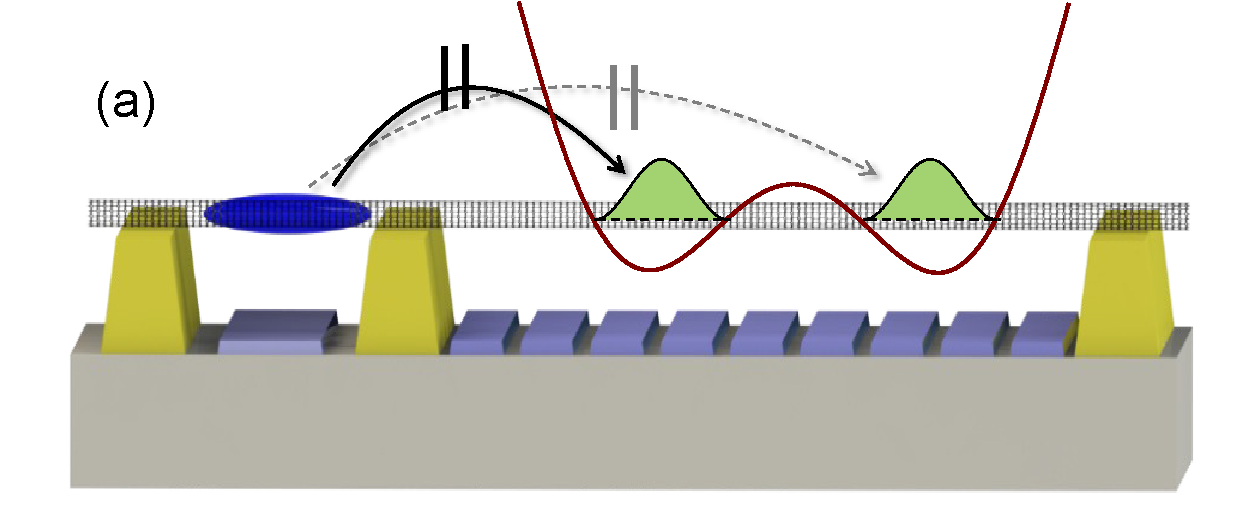
\includegraphics[width=0.9\columnwidth]{sketch_experiment_v2.pdf} %sketch_experiment_v3.png}
	 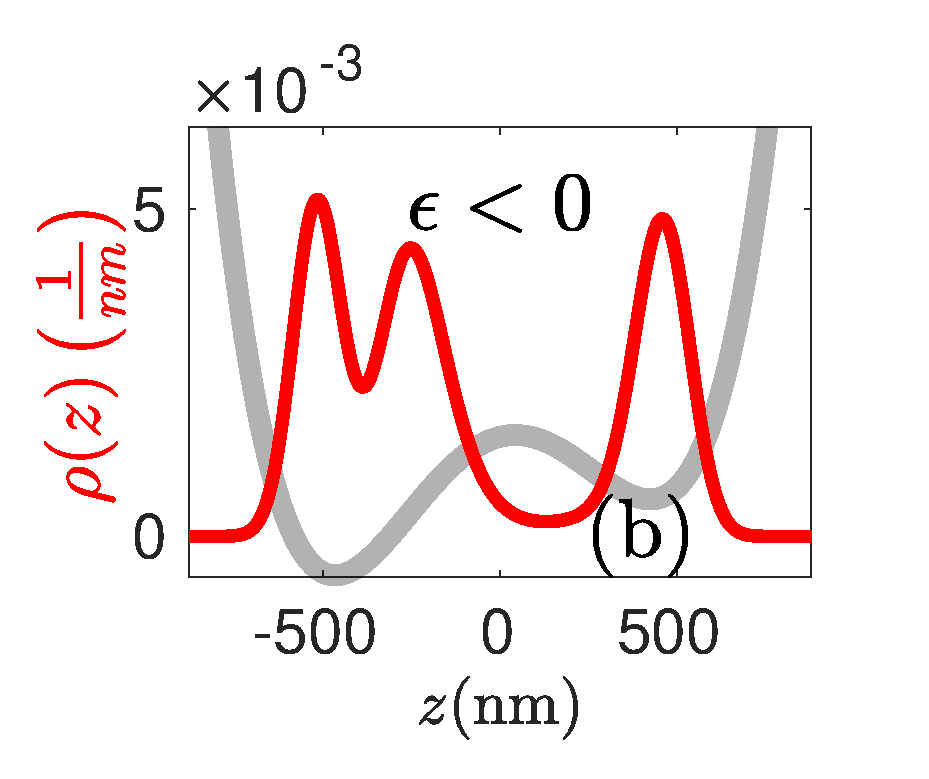
\includegraphics[width=0.49\columnwidth]{Fig_WaveFunction_Potential_NegEps_normalized.pdf}
     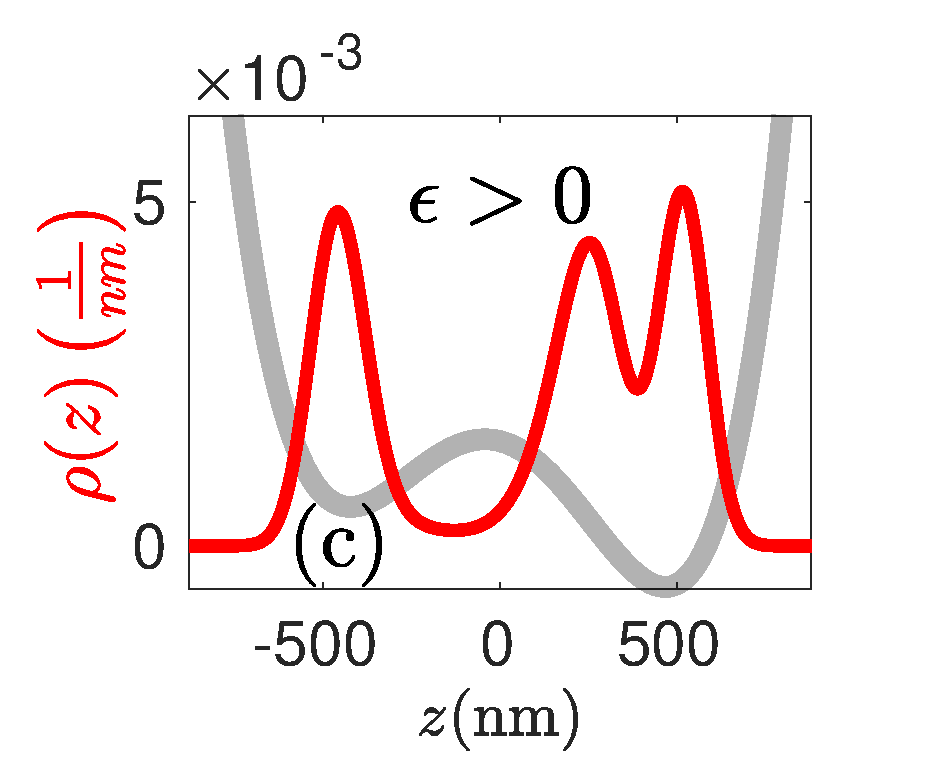
\includegraphics[width=0.49\columnwidth]{Fig_WaveFunction_Potential_PosEps_normalized.pdf}
	
    \end{center}
    \caption{(a)   Experimental setup of Ref.~\cite{Shapir.2019} used to detect 
	 collective tunneling. The bottom gates under the nanotube  are used to shape the double well potential, 
	 the left-hand-side quantum dot (dark blue)  serves as a charge detector.
	 (b) and (c) Ground state charge densities (red) from exact diagonalization for a system of three electrons  in a double well potential (grey).  A single electron moves between the two sides upon changing the asymmetry. The charge density displays a crystalline structure 
	 due to the strong Coulomb interaction ($\eta=20$ in Eq.~\eqref{eq:Hamiltonian_2}) .}
     \label{fig:experimental_setup}
\end{figure}




%The lattice spacing is approximately $\sim n^{-1}$. Therefore,  the formation of the Wigner crystal state can be determined by using the dimensionless ratio $r_s = (n a_B)^{-1}$, where $r_s\gg 1$ indicates the formation of the Wigner 
%crystal, while in  the oposite limit, i.e. $r_s\ll 1$,  the interactions are weak, and as
%the temperature is lowered, a Luttinger liquid state may emerge~\cite{Bockrath.1999, Levitov.2003}. 
%Initially, the observation of Wigner crystals has been observed to occurr on the surface of liquid helium~\cite{CRANDALL1971404, Grimes.1979}. Since then, they have been observed in various systems, such as two-dimensional electron gases that are confined to semiconductor heterostructures~\cite{Goldman.1990,Zhou2020}, and certain materials like transition metal dichalcogenide superlattices~\cite{Regan2020, Xu2020, Li2021}



In the present work we investigate theoretically  the collective tunneling of strongly interacting charged particles 
in the potential $V(z)$. Such collective tunneling occurs for an odd number of particles. Then the classical 
ground state of the particles is twofold generated in a symmetrical potential, but quantum tunneling allows for the hybridization 
of these two states, and splits their energy. However, as demonstrated experimentally \cite{Shapir.2019}, due to 
the strong Coulomb interaction, moving just one charge from one side of the barrier to the other 
is accompanied by the reordering of charges and a collective motion of all particles. 

The theoretical study of this phenomenon is rather challenging in the strongly interacting regime,
where usual quantum chemistry approaches break down \cite{RontaniPRB2010}.  We apply a combination of three 
different methods. In the deep tunneling regime an instanton approach can be used \cite{Milnikov.2001}. Incorporating 
quantum fluctuations turns out to be crucial  (as well as a technical challenge)  in the quantum tunneling regime. 
Unfortunately, most of the experimental data turn out to be in the intermediate region, where instanton theory is inapplicable. 
To capture the physics in this  regime, too, we perform (restricted)  exact diagonalization calculations and compare these with 
Density Renormalization Group (DMRG) based computations. These three approaches provide us a 
consistent  picture, confirm the presence of collective tunneling, and are in good agreement 
 with the experimental data.

 The paper is organized as follows: In Section~\ref{sec:modeling} we outline the 
basic model used to describe the experimental setup of Ref.~\cite{Shapir.2019}. 
 Section~\ref{sec:numerics} is devoted to the  discussion of the three complementary theoretical methods used in this work.
Our results are presented in Section~\ref{sec:comparison}, along with a detailed comparison with 
 the experimental data. Our conclusions are summarized  in Section~\ref{sec:conclusions}, while  some technical details of the 
 instanton calculation are described in  Appendix~\ref{app:prefactor}.


%\section{Key results}\label{sec:results}

\section{Modelling the experimental setup}\label{sec:experiment}
\label{sec:modeling} 

To observe the Wigner crystal regime in a carbon nanotube, the mass  of the charge carriers 
needs to be as large as possible, and their interaction as strong as possible. The
Wigner crystal regime is therefore ideally observed in suspended small diameter semiconducting 
nanotubes with large gaps, as the ones used in Refs.~\cite{Shapir.2019,Deshpande.2008}. 
Electrons  confined to  such nanotubes are  very well described by the effective  Hamiltonian 
\begin{gather}\label{eq:Hamiltonian_1}
H = \sum_{i = 1}^\n \left[ -\frac{\hbar^2}{2m^*}\frac{\partial^2}{\partial z_i^2} + V(z_i) \right] + \sum_{i<j}^\n \frac{e^2}{4 \pi \varepsilon_0}\frac{1}{\left| z_i - z_j  \right|},
\end{gather}
with $m^*$ the effective mass of the electrons (holes) in the nanotube, and $V(z)$ the confining potential, Eq.~\eqref{eq:potential}.
The spin $\sigma$ and the chirality $\tau$ of the particles do not appear  in this Hamiltonian~\cite{Charlier.2007}. 
They play an important role at larger electron densities~\cite{Sarkany.2017}. 
 However, since  the tunneling experiments studied here and in Ref.~\cite{Shapir.2019} are 
performed in the spin incoherent regime~\cite{Fiete2007}, here we  neglect them, and 
consider simply interacting spinless fermions. 
We also disregard the impact of spin-orbit interaction,  having 
a mild effect on the measured charge densities or the interaction energies. These, however, 
modify the structure of  spin excitations at very low temperatures or in the cross-over 
regime, where the Wigner starts to melt and the role of exchange interaction becomes 
important~\cite{Sarkany.2017}. 



Usually, the strength of electron-electron interaction  in a homogeneous, $d$-dimensional electron gas
is characterized by the parameter $r_s=n^{-1/d}/a_B$,   the ratio of the typical distance between charge 
carriers and the Bohr radius,  $a_B = \hbar^2 \varepsilon/me^2$. At $r_s\approx 1$
the electrons' kinetic energy is approximately the same as their potential energy, while for $r_s\gg 1$ the 
interaction energy dominates. It is in the latter regime that the Wigner crystal emerges. 

In a confined potential, however, the concept of $r_s$ is not particularly useful.
There the confining potential sets a typical length scale, which in our case is simply 
the oscillator length of the quartic potential ($a = c=0$), 
\begin{equation}
	l_d = \left( \frac{\hbar^2}{m^* b} \right)^{1/6}.
\end{equation}
Introducing  the corresponding dimensionless coordinates, $z\to \chi = z/l_d$, defines then 
the natural energy scale of the problem, 
\begin{equation}
	E_0 = \frac{\hbar^2}{m^* l_d^2}\;,
\end{equation}
and leads to the definition of the dimensionless  strength of the Coulomb interaction, 
\begin{gather}
	\eta = \frac{l_d}{a_B} = \frac{m^* e^2}{\varepsilon \, \hbar^2}\left ( \frac{\hbar^2}{m^*b}\right )^{1/6}.
\label{eq:eta}	
\end{gather}
For the nanotube investigated here and in Ref.~\cite{Shapir.2019} we obtain 
 \begin{eqnarray}
 l_d\approx 160 \,{\rm{ nm}}, \phantom{22}
 E_0 %\approx 0.48 \,{\rm{ meV}} 
 \approx 5.56\, {\rm{ K}}, \phantom{22}
 \eta \approx 20, 
 \end{eqnarray}
the latter signaling an extremely strong Coulomb interaction. 


%\begin{figure}[h!]
%    \begin{center}
%     \includegraphics[width=1.0\columnwidth]{Experimental_gap_1.pdf}
%    \end{center}
%    \caption{ The experimental measurement of the polarizability as a function of the gate voltage $V_K$ is conducted using the charge detector. By adjusting the voltage $V_K$, the height of the tunneling barrier can be controlled. The shaded area in the plot represents the onset of the tunneling regime for $N=3$, where the polarizability begins to exhibit exponential decay as $V_K$ increases. The arrow points to the offset voltage $V_0^{(3)}$, which marks the transition between the two regimes. }
%     \label{fig:Experimental_data}
%\end{figure}
%



  	
%\section{Model Hamiltonian}\label{sec:model}

In terms of these units, we  obtain  the dimensionless Hamiltonian
\begin{gather}\label{eq:Hamiltonian_2}
	\tilde{H} = \sum_{i = 1}^\n \left[ -\frac{1}{2}\frac{\partial^2}{\partial \chi_i^2} +\frac{1}{4} \chi_i^4 - \frac{\alpha}{2}\chi_i^2 -  \epsilon \chi_i \right] + \eta \sum_{i < j}^\n \frac{1}{\left| \chi_i - \chi_j  \right|},
\end{gather}
where the dimensionless parameter $\alpha= a \,l_d^2/E_0$  sets the height of the tunneling barrier between the two valleys, while 
$\epsilon= c\, l_d/E_0$ characterizes their bias.   

%
%For the scenario where an odd number of electrons, specifically $N\in\{1, 3, 5, 7\}$, are confined within the nanotube, we use the Hamiltonian described by Eq.~\eqref{eq:Hamiltonian_2} to calculate both the ground state energy and the first few excited states. This approach enables us to obtain the splitting spectrum that is observed in experiments and perform a quantitative analysis by comparing the numerical results with the experimental data.
%Numerically, we use a combination of approaches that includes the 
%exact diagonalization, density matrix renormalization group 
%and the instanton theory. All these approches will be discussed in Sec.~\ref{sec:numerics}. 






\section{Theoretical approaches}\label{sec:numerics}

Our goal is to compute the tunneling amplitude $\Delta$ of the crystal, 
i.e., the splitting of the two almost degenerate states for $N=\text{odd}$, and to investigate this 
tunnel splitting and the electrons' charge distribution as a function of the  potential  height $\alpha$, and the bias $\epsilon$.
The tunneling amplitude is inversely proportional to   the polarizability of the Wigner crystal at $T=0$ temperature, 
and is therefore directly accessible experimentally via polarization measurements, while  
charge distributions can be detected by an AFM-like method using 
a probe nanotube~\cite{Shapir.2019}.  


\subsection{Instanton theory}\label{sec:IT}



\begin{figure}[b!]
    \begin{center}
    	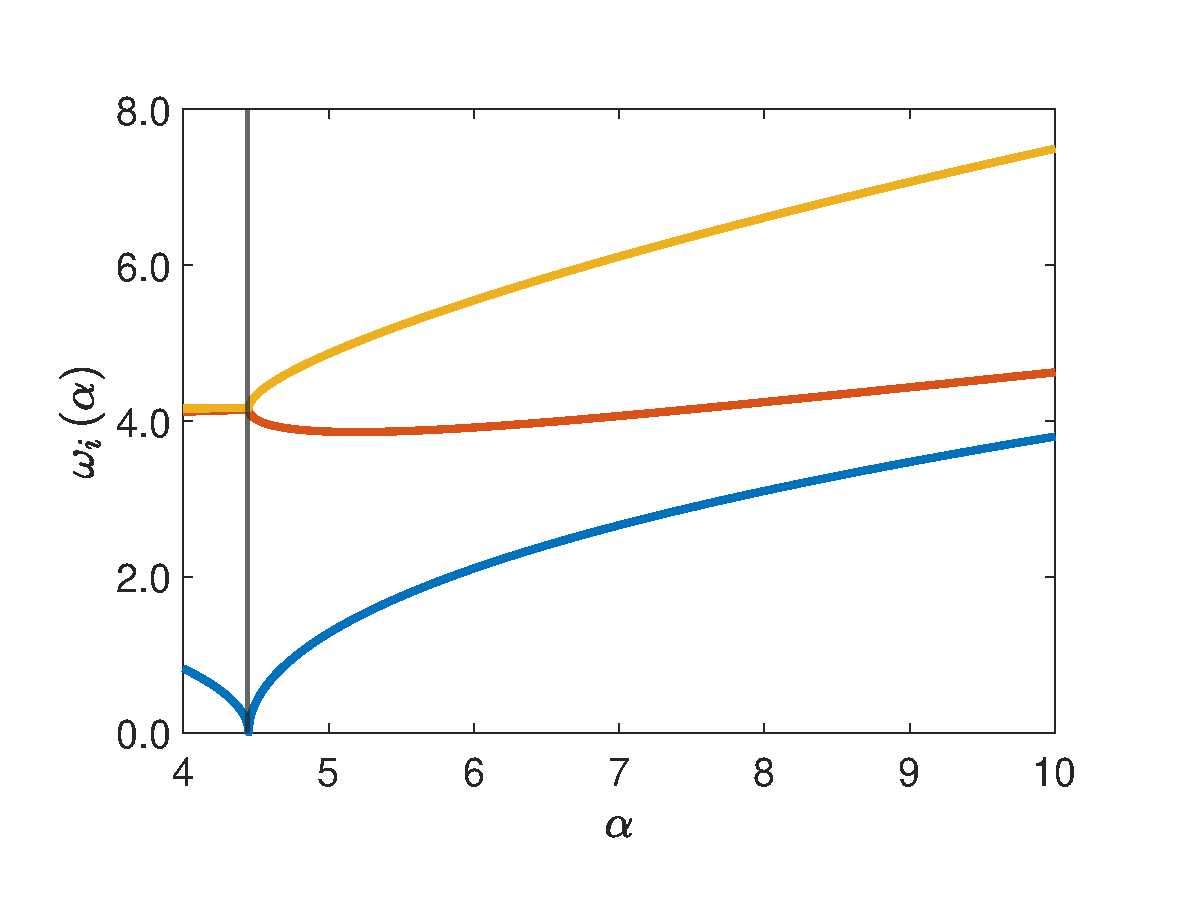
\includegraphics[width=0.9\columnwidth]{Fig_Freqs.pdf}		
     \caption{Soft modes $\omega_i$ as a function of $\alpha$, for $N=3$. The vertical line at $\alpha=\alpha_{cr} \approx 4.45$ marks the beginning of the tunneling regime. For $\alpha>\alpha_{cr}$ there are two independent equilibrium position, while for $\alpha<\alpha_{cr}$ only one, indicating the absence of the tunneling at small 
	 $\alpha$. }
     \label{fig:omega}
    \end{center}
\end{figure}  



We first consider the Wigner crystal tunneling problem by using the  instanton approach~\cite{Coleman.1988,Ciafaloni:1987qr, Grafke.2015,Richardson.2018,Milnikov.2001}.  Instanton theory  (IT)  is accurate  in 
the tunneling regime,  $\alpha\gg 0$,  however, it breaks down 
at small positive values, $\alpha\lesssim \alpha_\text{cr}$, with $\alpha_\text{cr}$ denoting the barrier height parameter, 
where tunneling sets in. 
 
 
 In the instanton approach, one considers the imaginary time  tunneling amplitude between two many-body  positions. 
  Tunneling appears as a classical motion of the 
 particles in imaginary time, and the tunneling amplitude is proportional to $\Delta \sim e^{-S_\text{inst}}$, with  $S_\text{inst}$
 the instanton action. Fluctuations around this classical path determine the amplitude of tunneling, i.e.,  the prefactor 
 in front of the exponential~\cite{Coleman.1988}. 

The energy splitting $\Delta$ of the lowest lying states can be obtained by computing the imaginary time  Feynman propagator, 
\begin{gather}
K(\mathbold{\chi}_0^\prime, \mathbold{\chi}_0, \tilde{\tau}) = \langle \mathbold{\chi}_0^\prime \vert \e^{- \ttau \,\tilde{H}} \vert \mathbold{\chi}_0 \rangle,
\label{eq:Feynman}
\end{gather}
between the minima $\mathbold{\chi}_0$ and  $\mathbold{\chi}_0^\prime$
of the many-body potential, 
\begin{gather}
	v_\n(\bchi) = \sum_{i=1}^\n \left(-\frac{\alpha}{2} \chi_i^2 + \frac{1}{4} \chi_i^4   \right) + \eta \sum_{i < j}^\n \frac{1}{|\chi_i - \chi_j |},\label{eq:v_N}
\end{gather}
with $\ttau$     the dimensionless imaginary propagation time measured in units of $  \hbar/E_0$. % and tunneling times, respectively.
One can  express  \eqref{eq:Feynman} as a path integral in terms of the imaginary time trajectories, $ \mathbold{\chi}( \ttau)$, 
which  are separated into a classical instanton trajectory, $\bchi_\text{cl}(\ttau) $, 
minimizing  the classical (Euclidean) action
\begin{equation}\label{eq:ImagAction}
	S_E[\bchi(\ttau)]  = S_0 \int_0^{T} {\rm{d}}   \ttau \Big\{ {1\over 2}\sum_{i = 1}^\n\Big( \frac{{\rm{d}} \chi_i}{{\rm{d}}  \ttau} \Big)^2 + v_\n(\bchi)   \Big \}.
\end{equation}
and small fluctuations around that,   $ \bchi(\ttau) = \bchi_\text{cl}(\ttau)  + \br(\ttau) $. 
The prefactor $S_0 = (l_d / E_0)^{3/2}$ emerges naturally, and denotes  the natural action 
unit in this problem, and ${T}$ denotes the tunneling time in units of $\hbar/E_0$. 
Expanding the action to second order in $ \br(\tau) $  leads to the expression
 \begin{gather}
	K(\bchi_0', \bchi_0, \tT) \approx 
	 e^{-S_{\text{inst}}} \int_{\br(0) = 0}^{\br(\tT) = 0} \cD\br \exp  \Big\{ \frac{1}{2} \int_{0}^{\tT} {\rm{d}} \ttau \, 
	 \br(\ttau)\cdot\nonumber \\
	  \left[ -\partial^2_{\ttau}
	 + \partial \circ % \otimes
	 \partial \, v_\n(\bchi_{cl}(\ttau)) \right] 
	 \mathbold{r}(\ttau)
	\Big \}, 
	 \label{eq:K_full}
\end{gather}
with $S_{\text{inst}} = S_E [\bchi_\text{cl}(\ttau)]$ the instanton action, and the  integral accounting for quantum fluctuations around it.

We  determined the  initial and final equilibrium positions $\bchi_0$ and $\bchi_0'$ 
as well as the instanton trajectories  by applying a Monte Carlo simulated annealing  procedure~\cite{VANDERBILT1984259}. 
Fig.~\ref{fig:omega} shows the frequencies of  small vibrations around the minimum (minima) of 
$v_\n(\bchi)$ for $N=3$. The symmetrical position of the three particles becomes classically unstable 
at $\alpha^{N=3}_\text{cr}\approx {4.45}$,  the classical 
threshold  for collective tunneling.  For $\alpha<\alpha_\text{cr}$  the minimum energy configuration is unique,  
while for  $\alpha>\alpha_\text{cr}$ two equilibrium positions exist,  and tunneling becomes possible.  
The transition to the tunneling regime is marked by the softening of the lowest energy  mode. 
Interestingly,  the direction of this mode coincides with that of the instanton trajectory
for $\alpha>\alpha_\text{cr}$. 


%
\begin{figure}[t!]
    \begin{center}
    	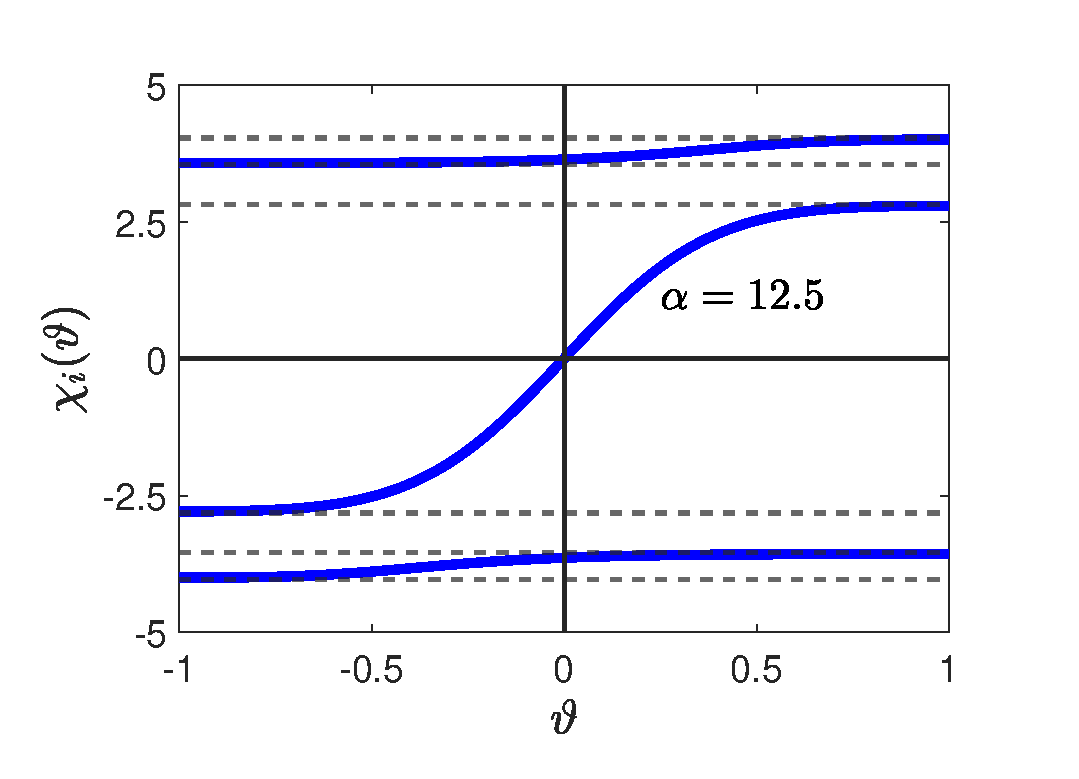
\includegraphics[width=0.95\columnwidth]{Fig_3Particle_Trajectory.pdf}		
     \caption{ Three particle imaginary time trajectories (blue) in the dimensionless units for a specific confinement parameter $\alpha = 12.5>\alpha_\text{cr}$ and $\eta = 20$. Dashed lines show the classical equilibrium positions or instanton turning points for the 3 particles. 
     %For $\alpha > \alpha_{cr}$ two stable positions exist, and the particles move between these by collective tunneling.
     }
     \label{fig:traj}
    \end{center}
\end{figure}  

A typical trajectory is displayed for $N=3$ particles in Fig.~\ref{fig:traj}, which demonstrates 
 collective tunneling. In our calculations,  we "compactify" time by introducing the parameter 
$\vartheta = \tanh( {\ttau}/{\ttau_0})$, and parametrize $\bchi$  by using $\vartheta$.
 Clearly, the middle electron tunnels through the potential barrier, while the outer 
 electrons  do not tunnel but  adjust their positions. 


The choice of $\ttau_0$ is important from the point of view of numerical accuracy. 
A small value of $\ttau_0$ increases the numerical accuracy in the tunneling region, 
while a large value of $\ttau_0\approx 5$ provides better resolution around the end of the trajectories.
Since  the primary contribution to the energy splitting arises from the region around $\ttau\approx 0$, 
a value $\ttau_0 \approx 0.5 $ turns out to be optimal for accurate calculations. 

% 
%In this new units, the Euclidean action can be expressed as
%\begin{gather}\label{eq:FinalAction}
%S_E = S_0 \int_{-1}^{1} {\rm{d}}\vartheta   \Big\{ \frac{(1 - \vartheta^2)}{2\varrho} \sum_{i = 1}^\n\Big( \frac{{\rm{d}}\chi_i}{{\rm{d}}\vartheta} \Big)^2 \\ \nonumber
%+  \frac{\varrho}{1 - \vartheta^2} v_\n(\bchi) \Big \}.
%\end{gather}
%



\begin{figure}[b!]
	\begin{center}
		%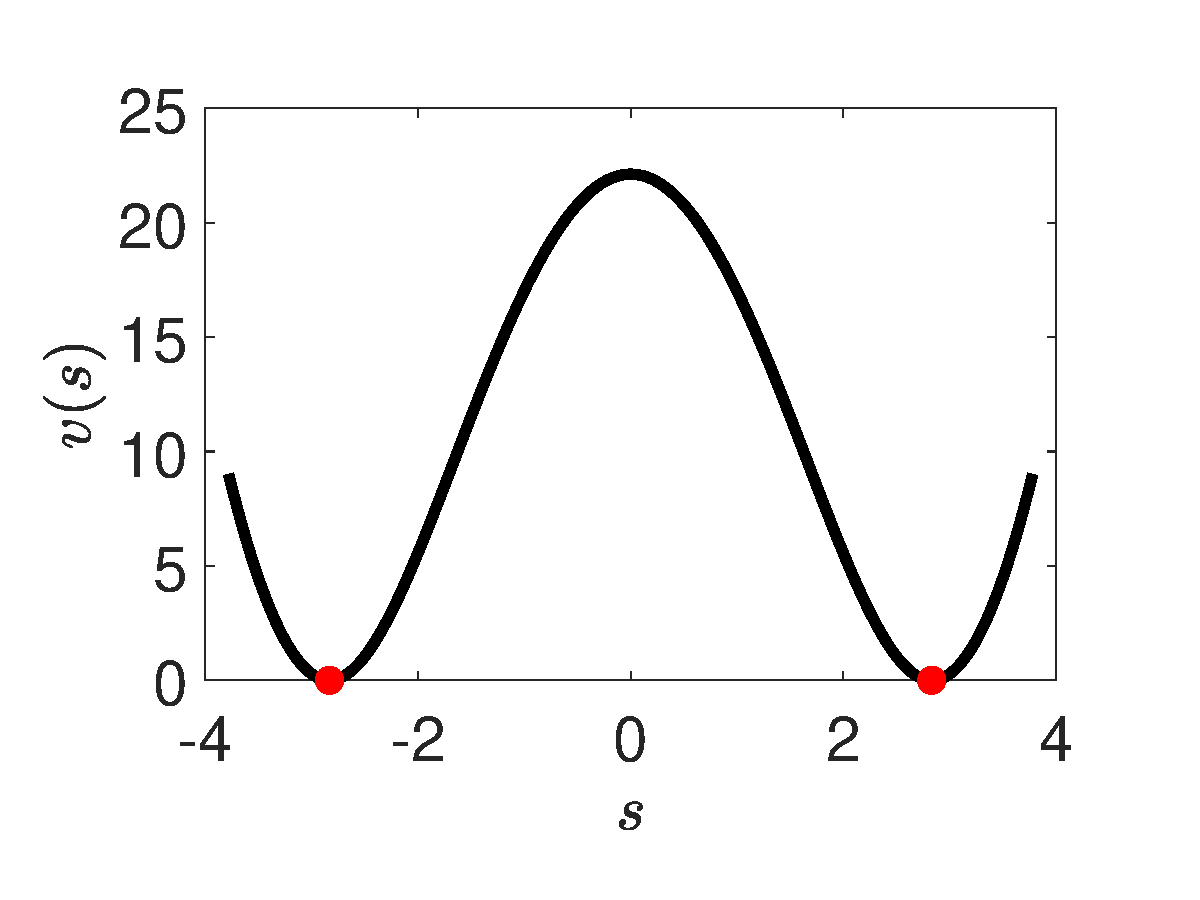
\includegraphics[width=0.9\columnwidth]{SupMatFig_EffectivePotential.pdf}
		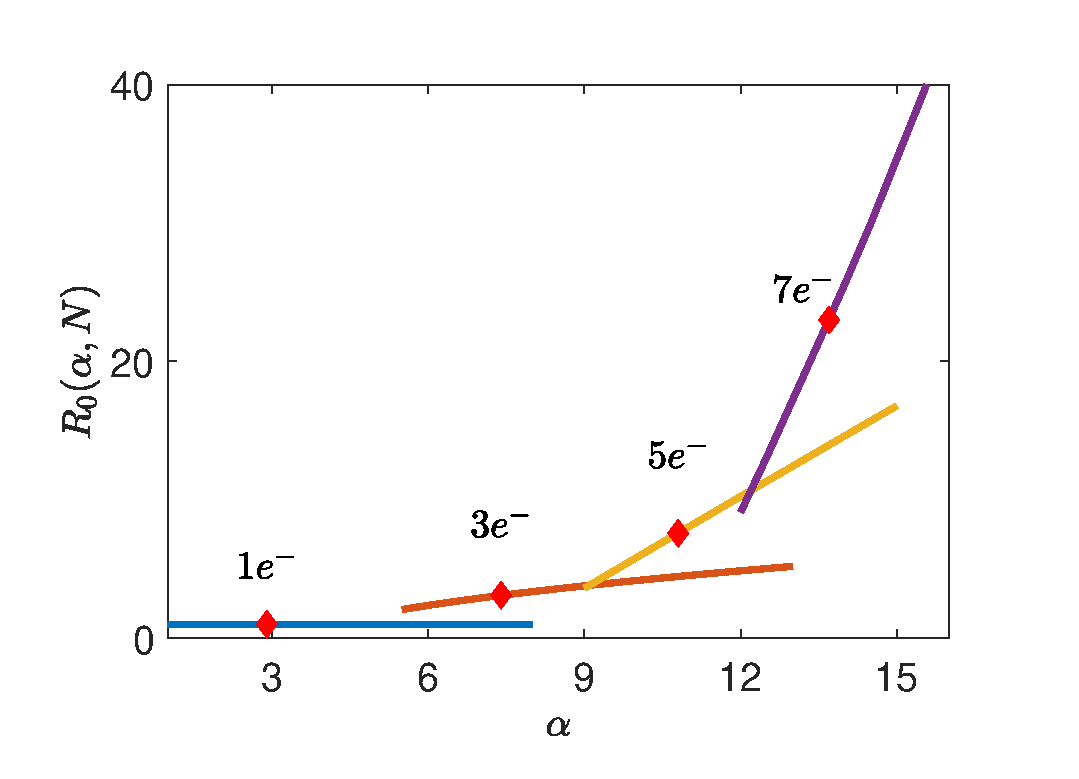
\includegraphics[width=0.95\columnwidth]{Fig_perpfactors.pdf}
		 \caption{
			%Top: Effective one-dimensional potential $v(s)$ for $N = 3$ particles, with $ds^2 = \sum_i d\chi_i^2$, for the arc length along the instanton trajectory for $\alpha = 10.5$ and $\eta = 20$. Red dots mark the classical turning points for the tunneling. Bottom: 
			Renormalization factor $ R_0(\alpha, N)$ as function of $\alpha$ for $N \in  \{1, 3, 5, 7\}$. 
			On each line, the diamond symbols mark the beginning of the quantum tunneling regime.  
			%Separate lines corresponds to a different $N$, as indicated.
			}
			\label{fig:R0}		
	\end{center}
\end{figure}

% Despite Eq.~\eqref{eq:FinalAction} shows divergent behaviour at the boundary of the integration domain, it is evident that the displacement of the quartic potential, such that the equilirium configuration's energy is zero, leads to the vanishing of the divergencies. Furthermore, as a known initial condition, the actions kinetic part vanishes exponentially at the boundaries.
%The propagation kernel naturally contains a number of symmetries, which we explicitly incorporated in order to stabilize the numerical solution. For a single particle, it exhibits the typical time reversal symmetry (T-symmetry). 
%When collective tunneling occurs, it exhibits the $RT$-symmetry, where $R$ is the reflection operator with regard to the particle $N+1 \over 2$ that is located in the center. This is in accordance with the requirements $\chi_{N+1 \over 2}(\vartheta)=-\chi_{N+1 \over 2}(-\vartheta)$ and $\chi_{N-i}(\vartheta)=-\chi_i(-\vartheta)$.
%To produce more trustworthy trajectories, we further enforce the restriction $\chi_{N+1 \over 2} (\vartheta=0) = 0$. 
%



%

% Given that the propagator yields equivalent probabilities to both the instanton (left-to-right tunneling) and anti-instanton (right-to-left tunneling) solutions of the Hamiltonian, one may impose symmetry constraints on the particle trajectories. Specifically, one may allow the middle particle's trajectory to evolve freely during the simulated annealing process between $\vartheta=-1$ and the time at which it reaches the midpoint of the potential barriers. Subsequently, one may apply the condition $\chi_{\rm{middle}}(\vartheta)=-\chi_{\rm{middle}}(-\vartheta)$ to ensure symmetry. Similar constraints may be applied to the trajectories of other particles by enforcing $\chi_{i}(\vartheta)=-\chi_{n-i}(-\vartheta)$. Furthermore the time corresponding to reaching the middle point of the potential can be also fixed as $\chi_{\rm{middle}}(\vartheta_0) = 0$ at $\vartheta_0 = 0$, without which the simulated annealing produces unreliable trajectories. For such trajectories see \ref{fig:traj}.top figure. An additional advantageous approach is to contemplate the non-interacting solution to the \eqref{FinalAction} equation (with the interacting equilibrium configuration as boundary condition) as a viable approximation of the particle trajectories. By leveraging these analytical paths as a starting point of the simulated annealing, computational efficiency can be enhanced.\\


Performing the Gaussian integral in Eq.~\eqref{eq:K_full} is a highly non-trivial task~\cite{mackenzie2000path,Milnikov.2001}. 
The procedure consists of introducing the arc length variable ${\rm d}s^2 = {\rm d}\bchi_\text{cl}^2 $
along the instanton trajectory, and $\n-1$ perpendicular coordinates. In this way, one describes the tunneling 
as a one-dimensional tunneling process in an effective potential $w(s)$, renormalized by  'perpendicular' 
quantum fluctuations (see Apendix~\ref{app:prefactor}). 
The tunneling amplitude is then expressed as
\begin{eqnarray}
\Delta &= &R_0 (\alpha, N) \, \Delta_{1}\,, 
\nonumber 
\\
\Delta_{1}& =&  \sqrt{\frac{4\omega_{\rm{soft}}}{\pi}} \sqrt{2 [v_{\n}^{\rm{max}} - v_{\n}^{\rm{min}}]} P[{\mathbold{\chi}}_{cl}(s)] e^{-S_E},
\label{eq:instanton}
\end{eqnarray}
with $\Delta_{1}$  associated with a one-dimensional motion in the effective double-well potential, 
and $R_0 (\alpha, N)$   the aforementioned renormalization factor~\cite{mackenzie2000path,Milnikov.2001} 
(see Appendix ~\ref{app:prefactor} for details). Here $\omega_{\rm{soft}}$ denotes the oscillation frequency 
at the initial position of the tunneling trajectory in the tunneling direction, and  $P\left[ \mathbold{\chi}_\text{cl}\right]$
is a renormalization factor associated with the effective one-dimensional motion. The  prefactor $R_0 $ is  equal to 1 for $N=1$, but it   becomes significant for $N\ge 3$ (see  
 Fig.~\ref{fig:R0}), and  exhibits a non-negligible $\alpha$ dependence.  Somewhat surprisingly, 
 quantum fluctuations seem to  increase the tunneling amplitude substantially, and  
 quantitative computations  must take them  into account. 

% \begin{itemize}
% \item {\color{red} Dont know where to put this: Note that the real time trajectories are expressable by analytic continuation.}
% \item Should I mention the results here, or it will be referenced later in the results section?
% \end{itemize}

\subsection{Density matrix renormalization group}\label{sec:DMRG}
As an alternative to instanton computations, we also performed density matrix renormalization group 
(DMRG) computations.  DMRG provides an accurate description of the intermediate tunneling 
regime, however, it fails in the deep tunneling regime, where we experience convergence problems. 

Originally, DMRG has been proposed as an efficient computational scheme 
for one-dimensional systems with short-ranged  interactions ~\cite{White.1992}, but
has  been extended later to systems with long-ranged interactions as well as to 
higher dimensional  lattices~\cite{Schollwock.2005}, and it has been 
reformulated more recently in a possibly more transparent way by using the language of 
matrix product states (MPS's)~\cite{SCHOLLWOCK201196,mcculloch2007density}. 

To perform  DMRG, we  express the Hamiltonian~\eqref{eq:Hamiltonian_2}  in a second quantized form. 
The key to efficient DMRG calculations   is to choose an appropriate basis in the strongly interacting limit studied here, 
$\eta \gg 1$.  The most natural choice of  harmonic oscillator basis functions centered at $\chi=0$, e.g., 
 is not able to reach this regime~\cite{RontaniPRB2010}. Here we perform calculations by using 
 an \emph{overcomplete adaptive basis}  with harmonic oscillator wave functions localized around the classical equilibrium 
 positions of the electrons~\cite{Shapir.2019}. 
 %To achieve this, we perform a Monte Carlo minimization of the classical 
 %potential energy~\eqref{eq:U} to obtain the classical configuration~\cite{VANDERBILT1984259} of the 
 %electrons and construct the local orbitals $\{\ket{\psi_j}\}$ at those positions.

%\begin{gather}
%	\tilde H_0 = \sum_{i = 1}^\n \left[ -\frac{1}{2}\frac{\partial^2}{\partial \chi_i^2} - \frac{\alpha}{2}\chi_i^2 + \frac{1}{4} \chi_i^4 + \epsilon \chi_i \right] \label{eq:H0},
%\end{gather}
%
%\begin{gather}
%	U = \eta \sum_{i < j}^\n \frac{1}{\left| \chi_i - \chi_j  \right|}.
%	\label{eq:U}
%\end{gather}
%
%To formulate 


In this basis, we  rewrite the Hamiltonian \eqref{eq:Hamiltonian_2} the second quantized form 
\begin{gather}
	\tilde H = \sum_{a,b} t_{ab} c^\dagger_a c_b + {1 \over 2} \sum_{a,b,c,d} V_{ab,cd} c^\dagger_a c^\dagger_b c_d c_c,
\end{gather}
where $t_{ab}$ stands for  the matrix elements of the non-interacting part of  \eqref{eq:Hamiltonian_2},
$t_{ab} = \langle \psi_a | \tilde H_0 | \psi_b \rangle$, while  $V_{ab,cd} = \langle \psi_a \psi_b | U | \psi_c \psi_d \rangle$ 
are  the matrix elements of the Coulomb interaction, $U=\eta/|\chi-\chi'|$ calculated within  
the single particle wave functions described above. The computation of   the matrix elements $V_{ab,cd}$ is numerically  demanding, but it can be speeded up 
by exploiting the  translational invariance of the Coulomb interaction.

%To compute the hopping amplitudes, it requires only a single integration, while to calculate the Coulomb integrals $V_{ijkl}$, we utilize the translational invariance of the Coulomb interaction and apply Fast Fourier Transformation (FFT) algorithms\cite{rao2010fast}. This approach effectively reduces the number of integrations and implicitly the computational time. 

\begin{figure}[t!]
    \begin{center}
    	%\begin{tabular}{cc}
    		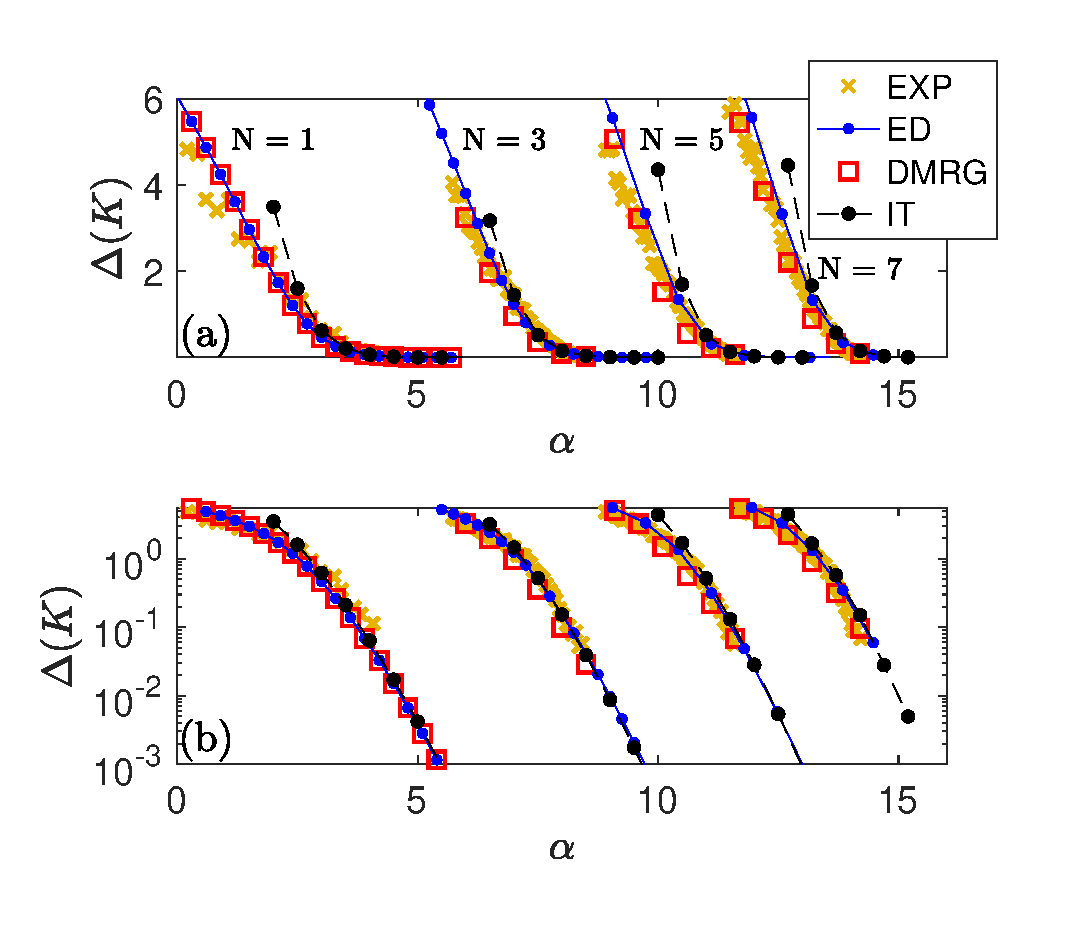
\includegraphics[width=0.95\columnwidth]{Fig_spectral_gap_exp_fitted_2.pdf}
     		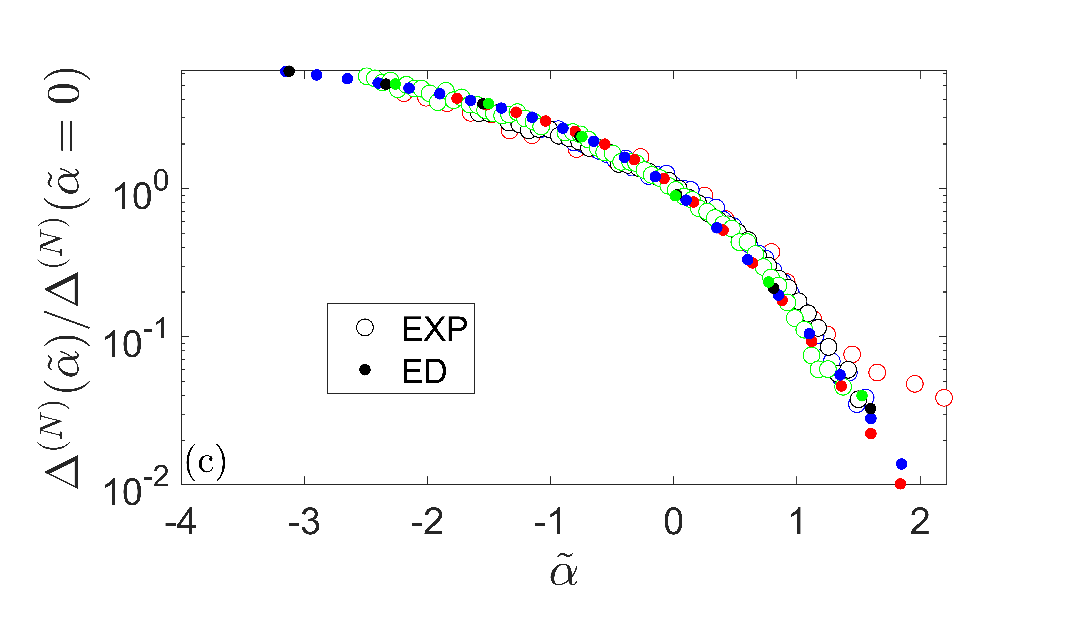
\includegraphics[width=0.95\columnwidth]{Fig_spectral_gap_exp_log_lin_shahal_scaling_log_v2.pdf}
    	%\end{tabular}
\caption{(a,b)  Numerically computed tunnel splitting on both linear  and logarithmic scales, compared 
with the rescaled experimental polarization data  (EXP).  Instanton theory captures  $\Delta$  accurately 
in the deep tunneling regime, where $\Delta$ is  suppressed exponentially by increasing barrier height (see  panel (b)).
 Each set of curves corresponds to a different number of electrons, $N$. 
 In panel (c), the data are scaled together and trace a single,   universal curve. 
 The tunneling regime starts at $\tilde\alpha\approx 0$.}    
     \label{fig:EXP_DMRG_ED_IT}
    \end{center}
\end{figure}    

For our computations,  we utilized the Budapest-DMRG code~\cite{Ors,legeza1996accuracy, Ors2016},
which allows us to treat long-range interactions efficiently and to take advantage of the $U(1)$ 
symmetry of the model associated with the conservation of the total charge as well as  the $Z_2$ 
symmetry associated with  parity. In our computations, we use a bond dimension of the order of   2048-4096,  and
an adaptive basis consisting of  $8-16$ 
orbitals/electron, depending on the number of electrons. 
We  computed the ground state energies in the even and odd parity sectors,  $E_{GS}^{(e)}$ and $E_{GS}^{(o)}$, and 
extracted the energy splitting
\begin{gather}
	\Delta  = |E_{GS}^{(e)}-E_{GS}^{(o)}|,\label{eq:gap}
\end{gather} 
identified as twice the tunneling amplitude in the tunneling regime. 
Typical results for $\Delta$ as well as  a comparison with the results of the  other  approaches 
we used are displayed in Fig.~\ref{fig:EXP_DMRG_ED_IT} as function of $\alpha$. Unfortunately, 
in the deep tunneling regime, where     $\Delta $ becomes
exponentially small, $\Delta\lesssim 10^{-3}$, 
we noticed that the convergence of DMRG was influenced by the choice of basis we utilized. Specifically, as we decreased $\alpha$, the states became increasingly localized, which led to convergence challenges for the desired accuracy. Although increasing the bond dimensions improves the calculations, it also demanded greater computational resources. Consequently, as an alternative approach, we employed complementary methods like restricted exact diagonalization or instanton theory to achieve accurate results.
Nevertheless, the range of applicability of DMRG overlaps with that of these methods, and 
enables us to obtain a complete description of the collective tunneling. 

\subsection{Restricted Exact Diagonalization}\label{sec:ED}
As a third,  complementary method, we also used the restricted exact diagonalization (ED),  which can be  utilized to determine the 
 eigenstates of relatively small quantum systems. Here we also  use it to benchmark the other two,  more sophisticated 
 methods.
 % ~\cite{Bohr_2006, Khemani.2016}. 
In this work, we  diagonalize the Hamiltonian~\eqref{eq:Hamiltonian_2} in real space. 

% $\{\ket{\bchi} = \{\chi_{i}\}_{i=1}^N\}$ basis.





For $N\in \{ 1,3\}$,  diagonalization is performed with a relatively large number of states,  $\sim 100$ for each particle, 
ensuring accurate ground state and a few excited state energies. However, for $N\in \{5,7\}$, the Hilbert space 
becomes too large, and a complete diagonalization  is impossible in practice. 
Nevertheless, a projected version of ED can be used even in these cases, 
where a restricted wave function is used, with electrons treated as distinguishable particles. 
This method reduces the size 
of the Hilbert space by 2-3 orders of magnitude, and can be used to study  up to $N=7$ electrons
 the low-energy spectrum  in the strongly interacting limit, 
where exchange processes are unimportant~\cite{SIMON1984101}. 


\section{Results and comparison with experimental data}
\label{sec:comparison}

\subsection{Polarization, polarizability, and tunneling amplitude}

%Potential_shift_n5_cropped
\begin{figure}[t!]
		\begin{center}
			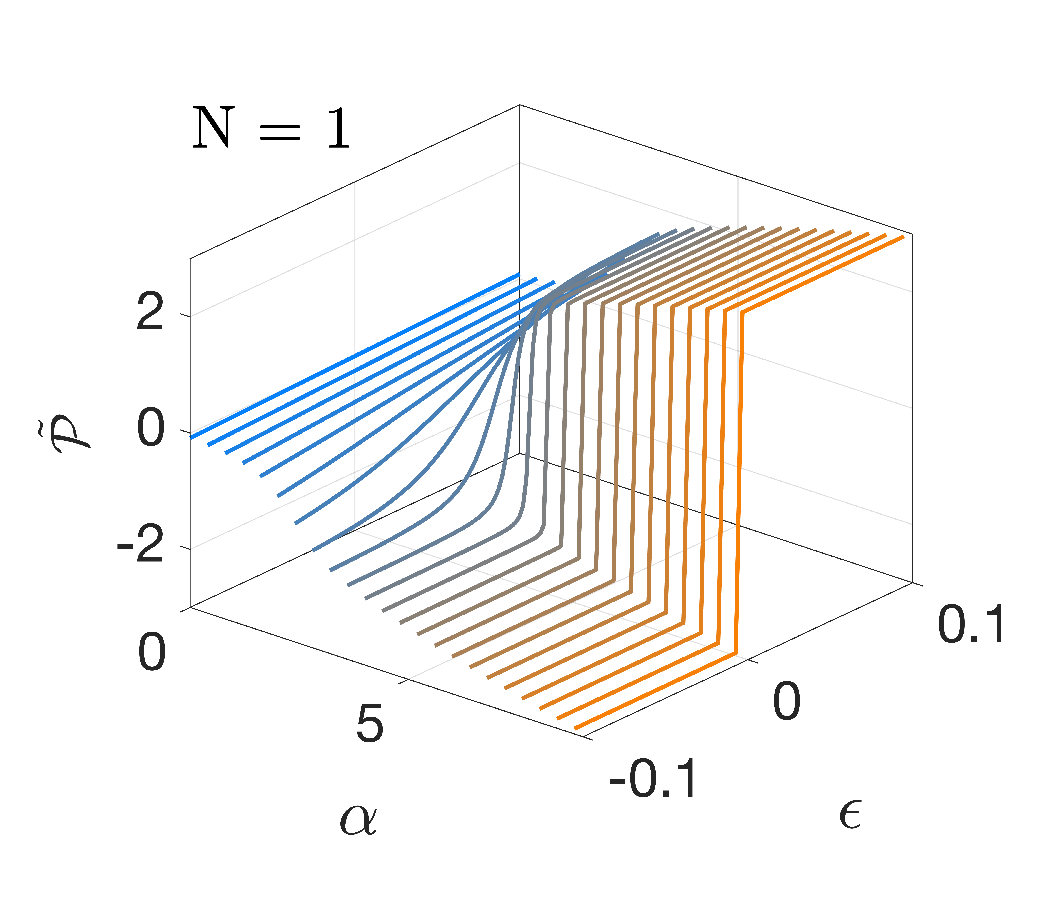
\includegraphics[width=0.49\columnwidth]{Fig_Polarization_3D_theor_1part_line.pdf}
			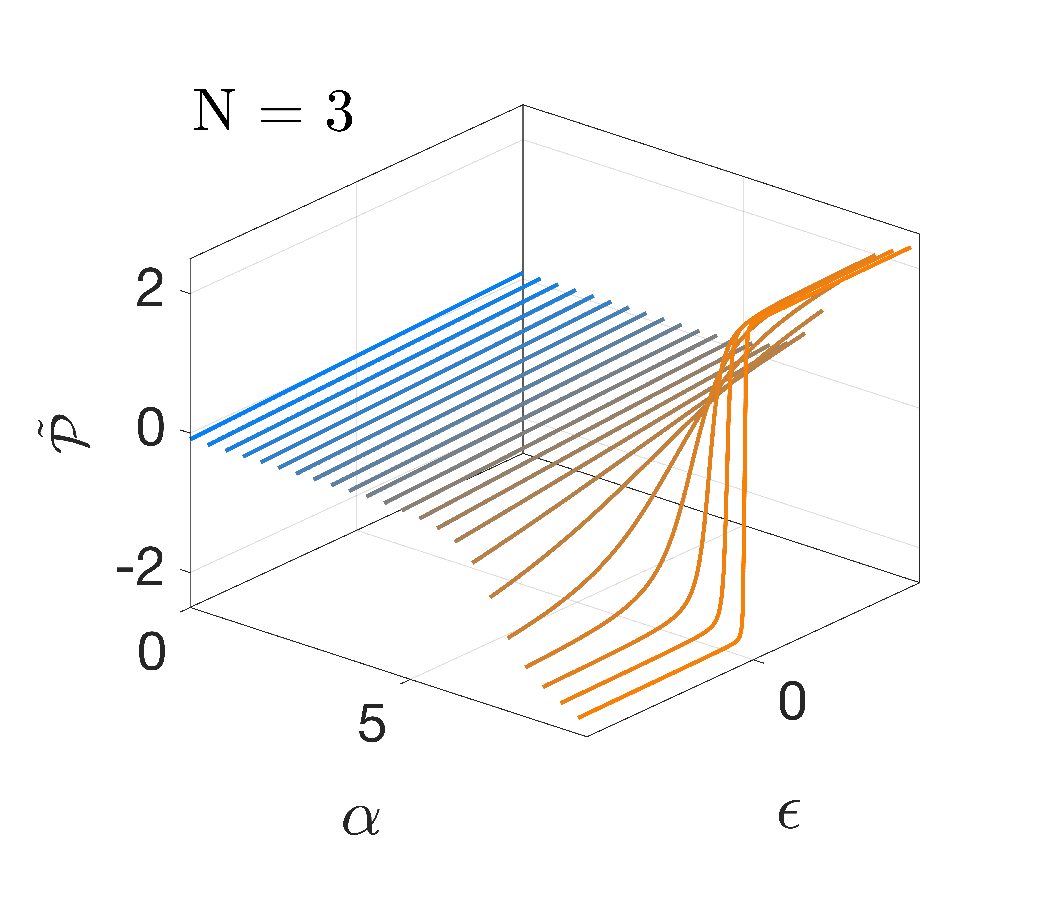
\includegraphics[width=0.49\columnwidth]{Fig_Polarization_3D_theor_3part_line.pdf}
			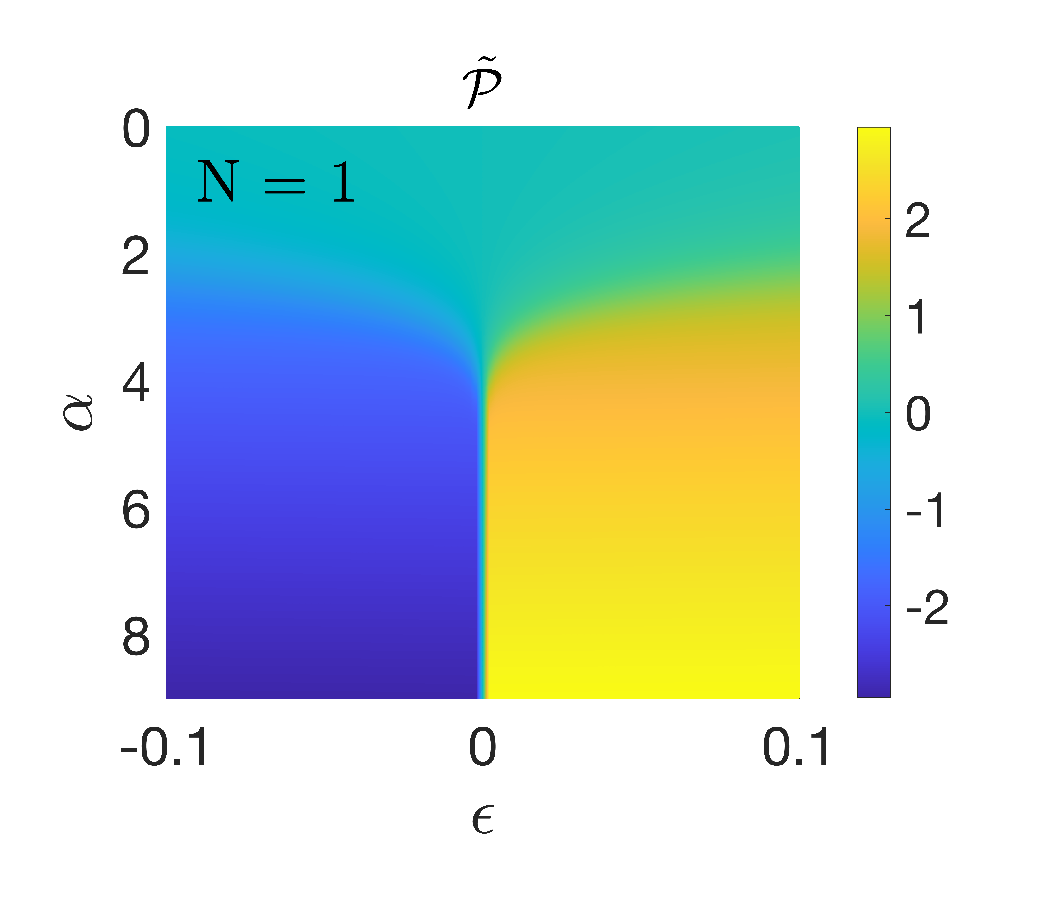
\includegraphics[width=0.49\columnwidth]{Fig_Polarization_3D_theor_1part.pdf}
			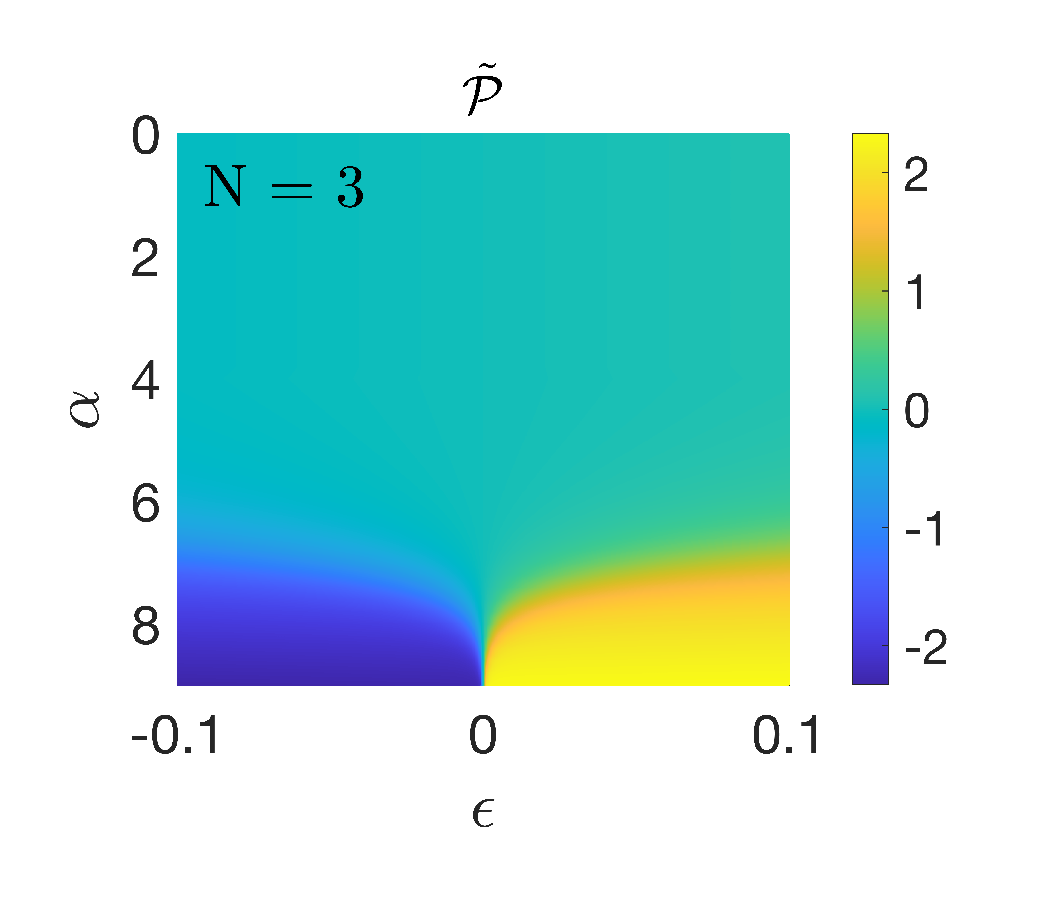
\includegraphics[width=0.49\columnwidth]{Fig_Polarization_3D_theor_3part.pdf}
		%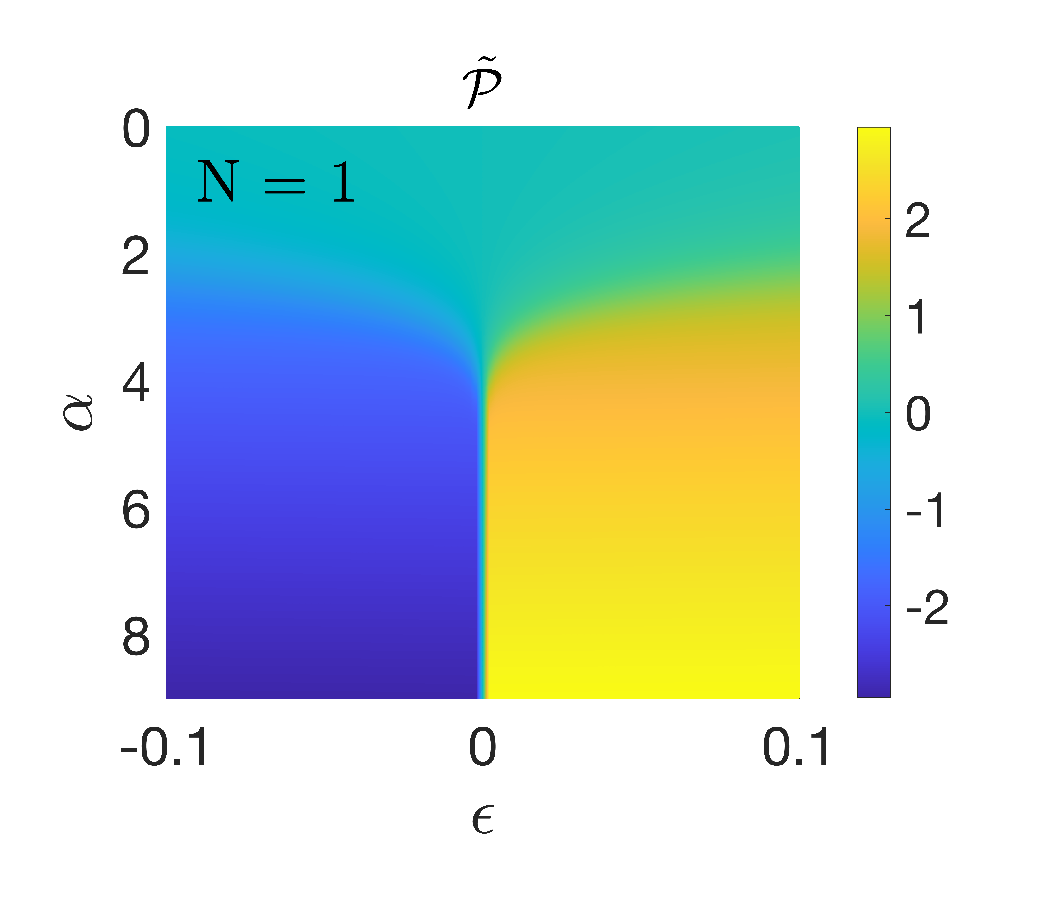
\includegraphics[width=0.65\columnwidth]{Fig_Polarization_3D_theor_1part}
		%\includegraphics[width=0.65\columnwidth]{Fig_Polarization_3D_theor_5part}
		 \caption{Density plots for the charge polarization $\tilde P(\alpha, \epsilon)$ represented as a function of $\alpha$ and $\epsilon$. The polarization is calculated for $N=1$ and $N=3$ electrons inside the confinement potential.}
		\end{center}
		\label{fig:polarization_comparison}
\end{figure}

The careful design and control in the experiments of Ref.~\cite{Shapir.2019} allows one to 
measure the polarization ${P}$ of the electrons on the nanotube as a function of the  applied bias 
($\epsilon$  in Eq.~\eqref{eq:Hamiltonian_2})  as well as  that of the height of the barrier, regulated by a back gate potential $V_K$. 
Such polarization results are displayed in Fig.~\ref{fig:polarization_comparison} along with our theoretical calculations for $N=3$.

In the theoretical computations in Fig.~\ref{fig:polarization_comparison}, we define the dimensionless polarization simply as
\begin{equation}
\tilde{P} (\alpha, \epsilon) = N \langle \chi\rangle = \int\limits {\rm d} \chi  \,\chi \,\rho (\chi, \alpha,\epsilon)   \;,
\label{eq:pol}
\end{equation}
with $ \rho (\chi, \alpha,\epsilon) $ the ground state charge density
\begin{equation}
\rho(\chi,\alpha, \epsilon) = \sum_{i=1}^\n \bra{\Psi}  \delta(\chi - \chi_i)\ket{\Psi},
\end{equation}
and  $\ket{\Psi} = \ket{\Psi(\bchi, \alpha, \epsilon)}$ the ground state wave function 
obtained using ED or DMRG. 





As one enters the quantum tunneling regime, the polarization displays a 
kink as a function of the  applied bias. This kink becomes sharper and sharper 
as  the barrier height increases,  clearly demonstrating that 
the broadening of the polarization jump in the experiments is not due to thermal fluctuations, but is 
dominated by \emph{quantum fluctuations} – excepting the very deep tunneling regime, where 
the transition becomes very sharp and its width is set by thermal fluctuations. 

In this quantum tunneling regime,  right at the transition, $\epsilon=0$, 
the polarizability  is inversely proportional to the tunneling amplitude, 
\be
\Pi = \frac{\partial {P}}{\partial \epsilon} \propto \frac 1 {\Delta}\;.
\ee
The precise prefactor here is  hard to determine, since it depends on the precise charge distribution 
before and after the tunneling. Also, although the response at the charge sensor is certainly 
proportional to the polarization, it depends on the capacitive coupling between 
the electrons at various positions and the charge sensor.
Nevertheless, the relation above  enables us to extract the tunneling amplitude as a function 
 of the shape of the barrier, apart from an overall scale. 

For a detailed comparison with the experiments,  we assumed that  there is a linear relation
between the voltage  $V_K$ and  the dimensionless parameter $\alpha$. This leads to the relations
\begin{eqnarray}
	\alpha^{(N)}  &=& \alpha_0^{(N)} +x^{(N)} \; (V_K - V_{0}^{(N)}),\nonumber\\
	\Delta^{(N)} &=&y^{(N)} \; \frac {\Pi^{(N)}(V_{0}^{(N)})} {\Pi^{(N)} (V_K)} .
	\label{eq:rescaling}
\end{eqnarray}
Here the parameters $\alpha_0^{(N)}$ 
%\approx \alpha_{cr}$  
and $V_{0}^{(N)}$ mark the threshold of tunneling regime, while $x^{(N)}$ and $y^{(N)}$ rescale the 
axes. We obtain a remarkably accurate fit
to the experiments, as displayed in Fig.~\ref{fig:EXP_DMRG_ED_IT}. Our fitting parameters are 
 enumerated  in Table~\ref{table:parameters}; both $\alpha_0^{(N)}$ and $x^{(N)}$ scale roughly 
 linearly with the threshold, $V_0^{(N)}$, while the overall  polarizability rescaling coefficient
 scales as $y^{(N)}\sim 1/N$.
 Interestingly, the data obtained for various $N$ values also display  a universal scaling when plotted as a 
function of $\tilde \alpha = \alpha-\alpha_0$, as demonstrated in Fig.~\ref{fig:EXP_DMRG_ED_IT}. 
%{\red\bf The rescaling factor $x$ is extremely large.} 
 
%It is worth noting that even though there is a slight difference between them, , both are indicating the onset of the tunneling regime. 
%
%
\begin{table}[t!]
	\begin{tabular}{|c|c|c|c|c|}
	\hline
	$N$ & $\alpha_0^{(N)}$   & $x^{(N)} \; [\text{meV}]^{-1}$ & $y^{(N)}\;\text{[meV]}$ & $V_0^{(N)} \;\text{[meV]}$ \\ \hline
	1 & 2.2 & 14.8   & 1    & 109     \\ \hline
	3 & 6.9  & 74.2  & 0.25 & 280     \\ \hline
	5 & 10.4 & 141.9  & 0.15 & 560    \\ \hline
	7 & 13.2  & 170.8  & 0.13 & 850    \\ \hline
	\end{tabular}
	\caption{List of rescaling parameters appearing in Eq.~\eqref{eq:rescaling}.
	}
	\label{table:parameters}
	\end{table}

%
%In Fig.~\ref{fig:EXP_DMRG_ED_IT} (a,b)
%we represent the experimentally rescaled polarizability  and the numerical results for the tunnel splitting
%as a function  of the confinement parameter $\alpha$. For the numerical data we present the results for all the three approaches that we discussed before which indicates a good agreement between them. Nevertheless, discrepancies are noticeable in the IT calculation for $\alpha\le \alpha_{cr}$, which is outside the tunneling regime where the IT technique is expected to be unsuccessful.

% \begin{align}
% {\text{"Universal scaling"}}\\
% v &= (V - \delta V_{\n})/V_\n \\
% \tilde{\Delta} &= \Delta\, f_\Delta \\
% \tilde{\alpha} &= (\alpha - \alpha_0^{(\n)}) f_{\alpha, \n} \\
% {\text{Scaling to }} \alpha \\
% \alpha(V) &= \delta\alpha_\n + \frac{1}{V_0} \left(V - \delta V_\n  \right)
% \end{align}
%
%
% 

\begin{figure}[t!]
    \begin{center}
     %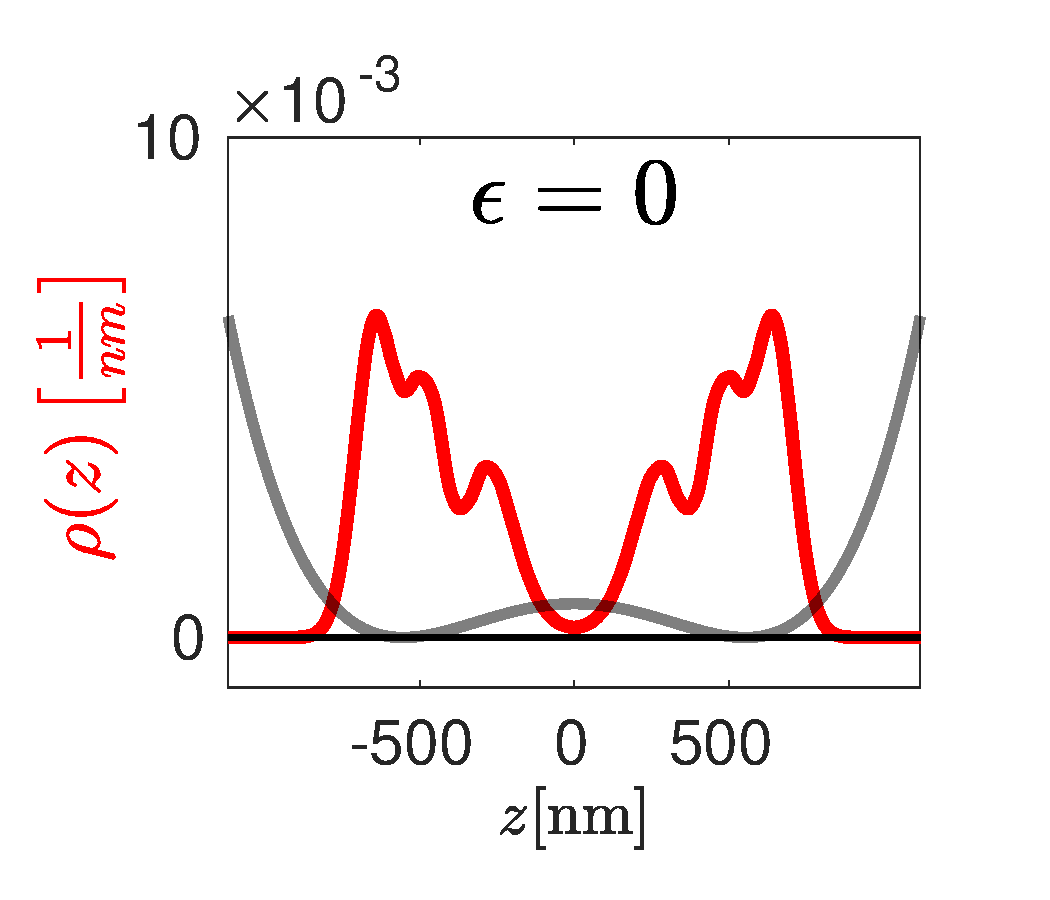
\includegraphics[width=0.48\columnwidth]{Fig_WaveFunction_Potential_eps1.pdf}
     %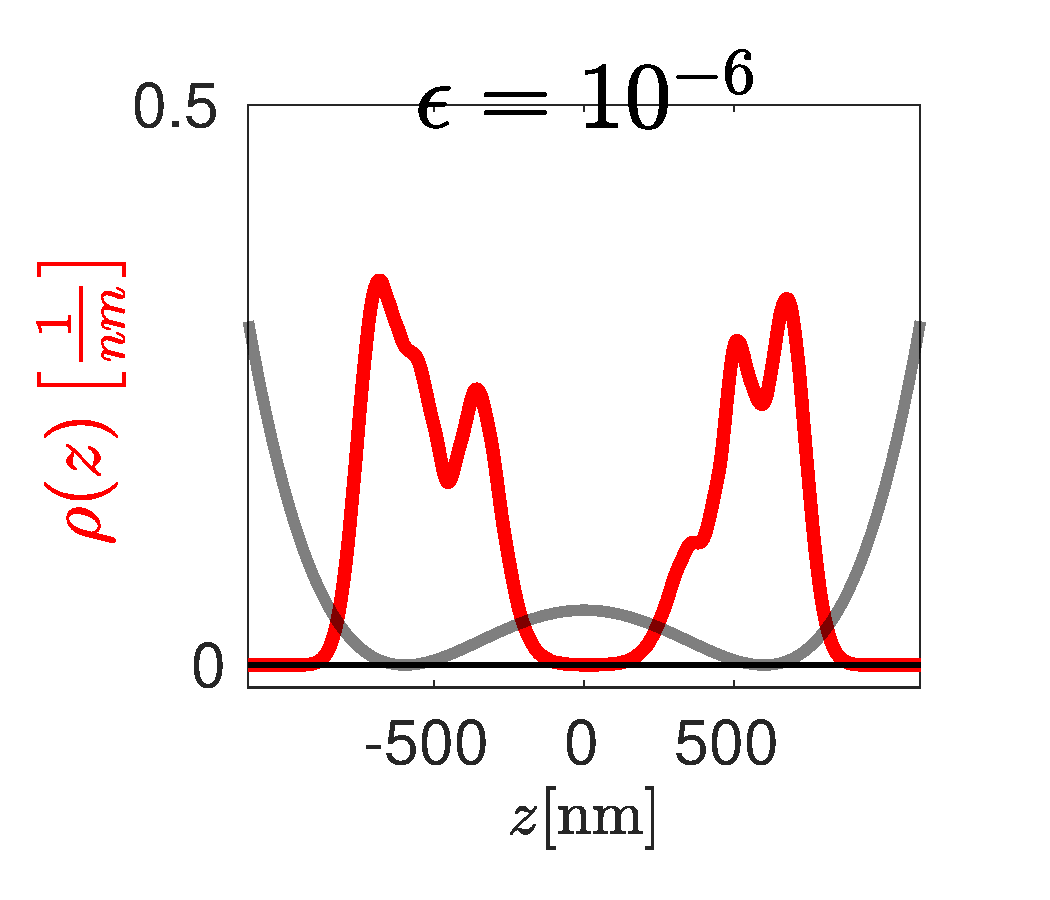
\includegraphics[width=0.48\columnwidth]{Fig_WaveFunction_Potential_eps2.pdf}\\
     %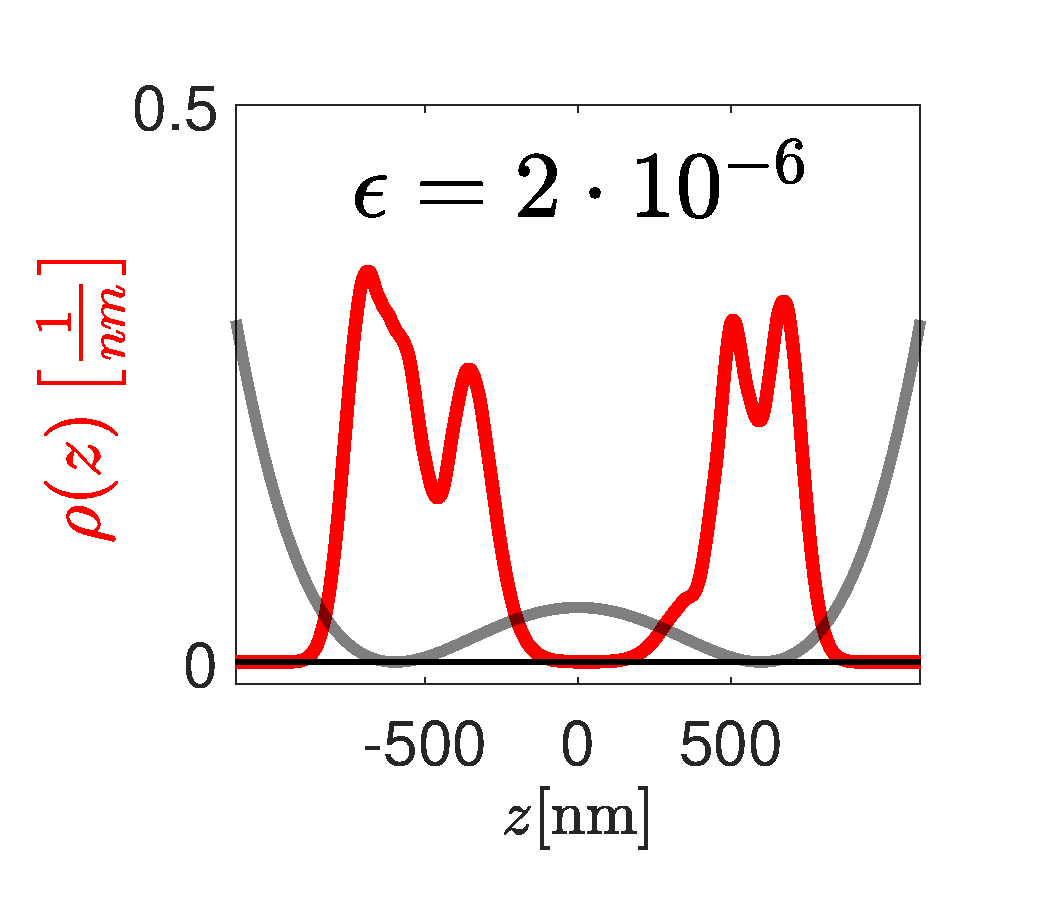
\includegraphics[width=0.48\columnwidth]{Fig_WaveFunction_Potential_eps3.pdf}
     %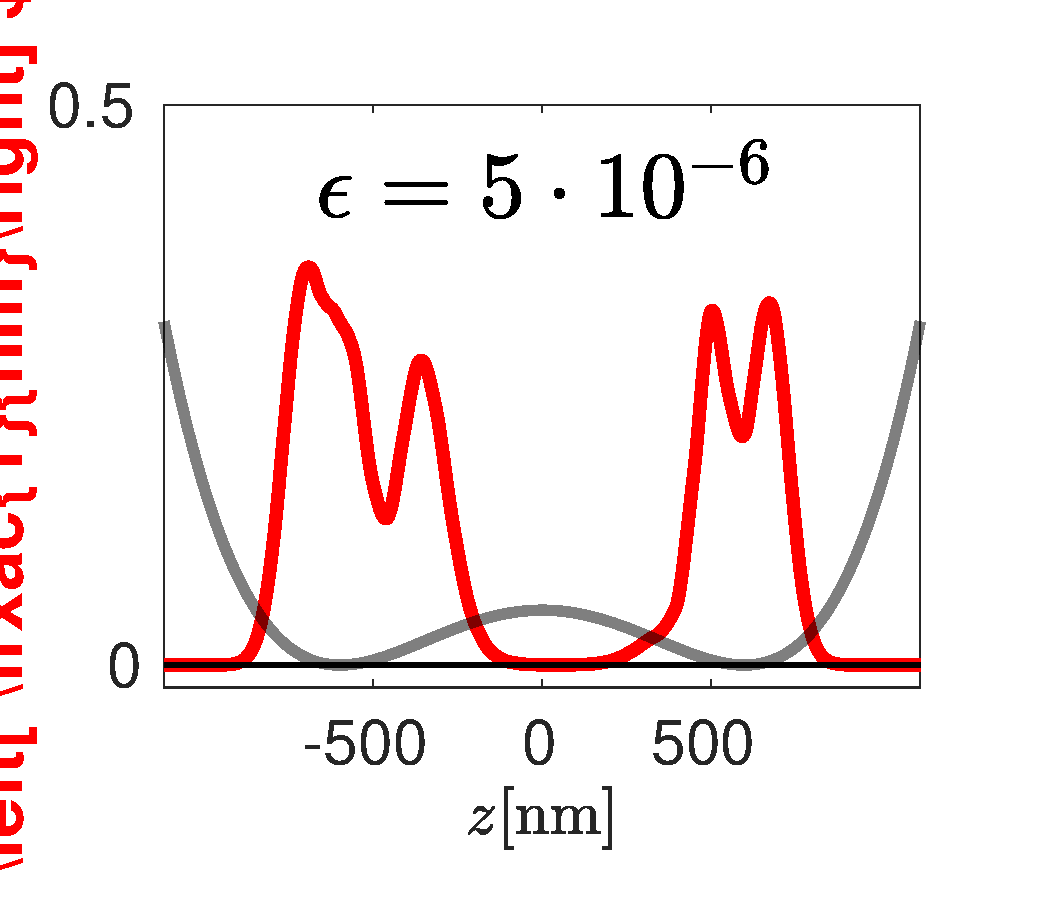
\includegraphics[width=00.48\columnwidth]{Fig_WaveFunction_Potential_eps4.pdf}
     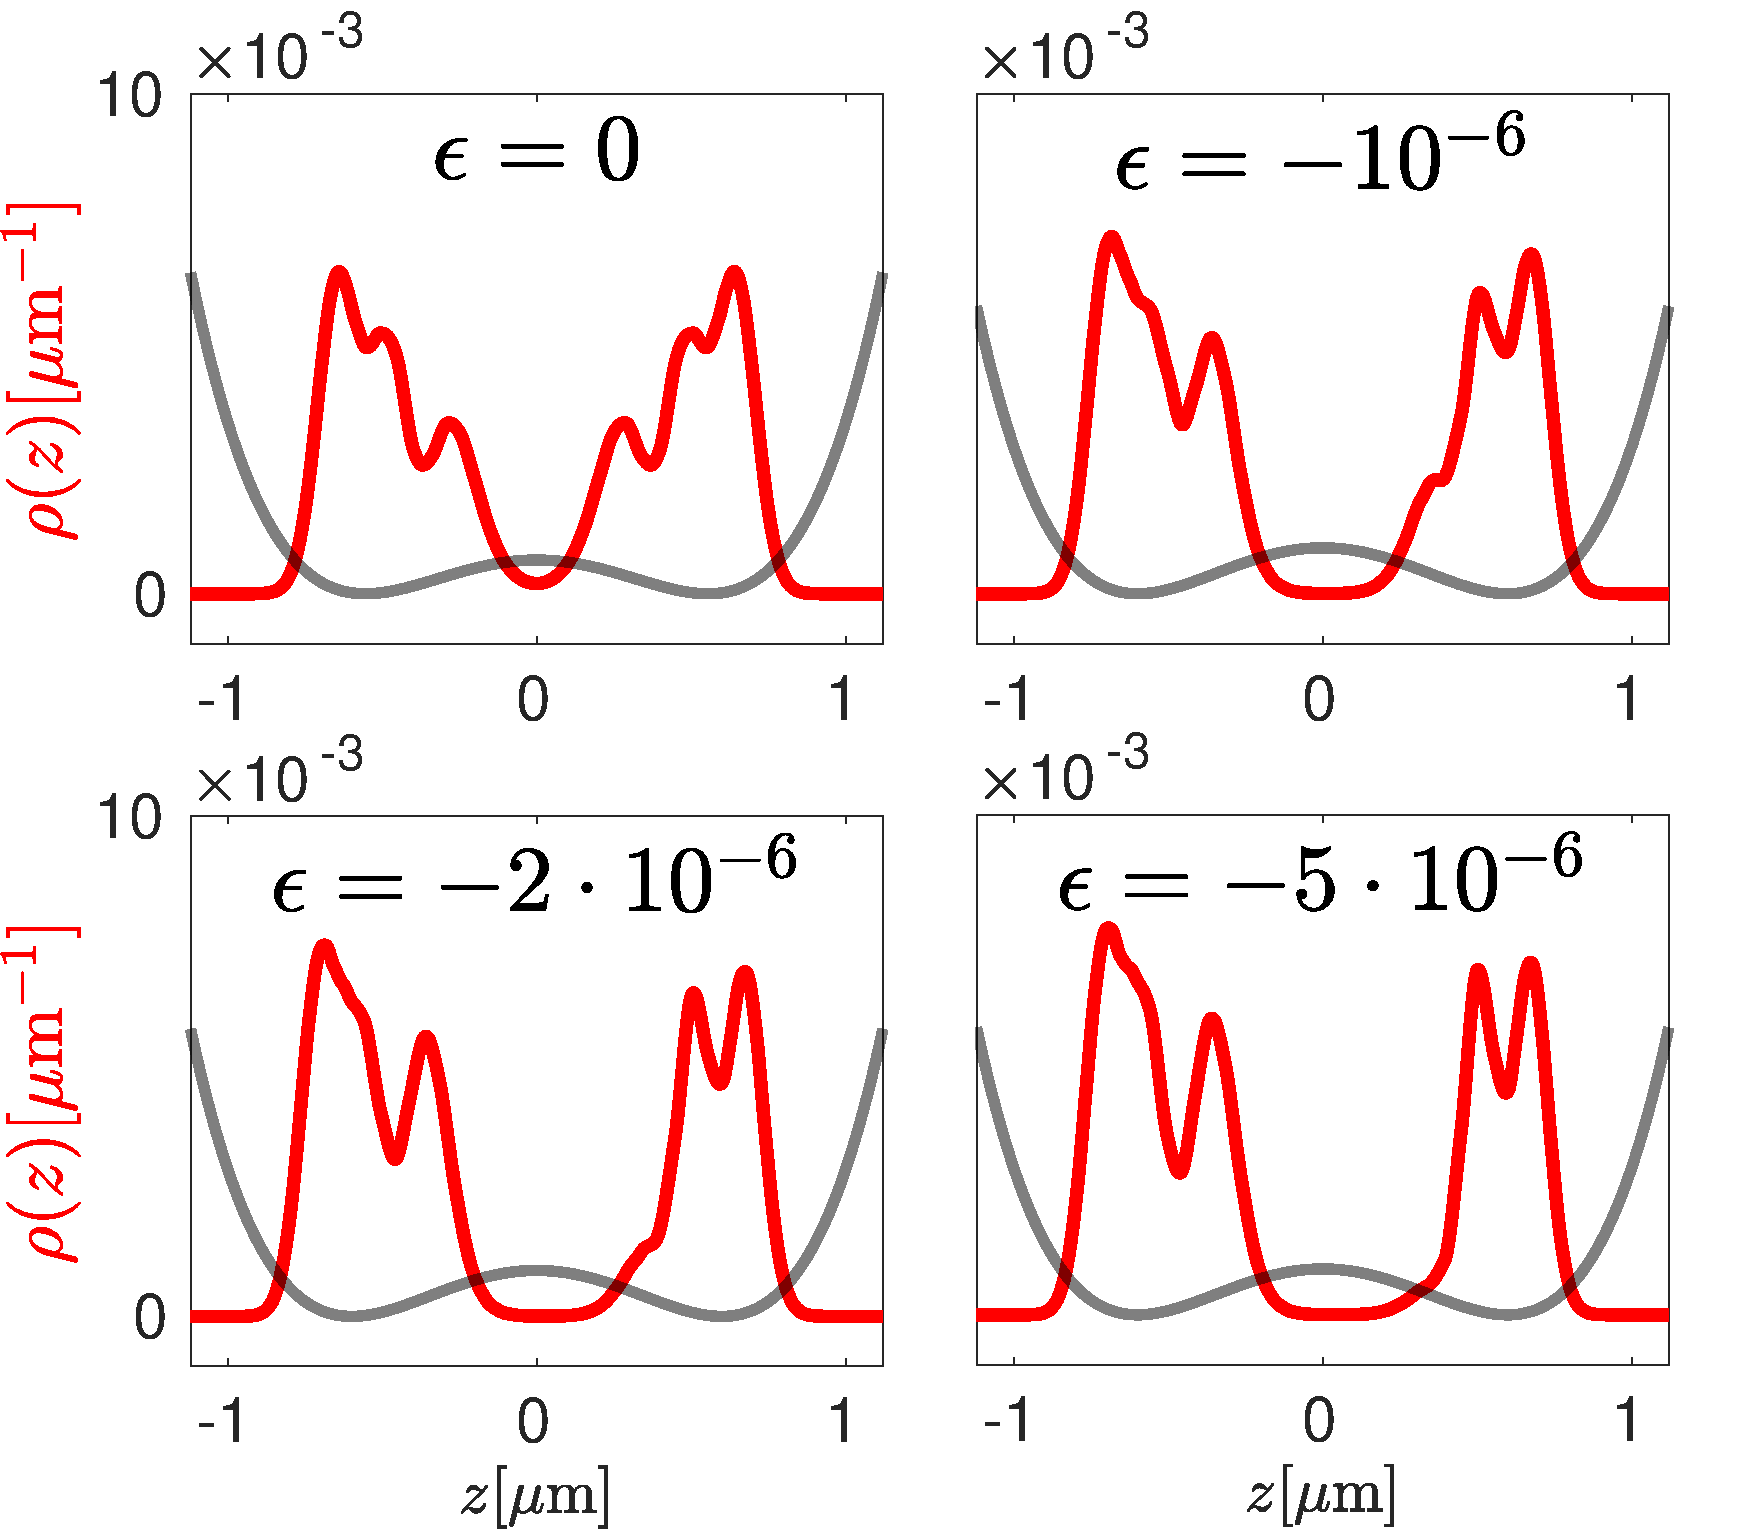
\includegraphics[width=\columnwidth]{FiveParticleDensitySeriesv2.pdf}
     \caption{
      \label{fig:charge_distribution_n5} Charge distribution profiles for $N = 5$ particles, with different $\epsilon$ values. At $\epsilon = 0$ the particle in the middle is represented on both sides of the potential barrier, while by increasing the linear detuning, we see that it slowly shifts to one side, changing the positions for the side particles as well.}
	  \label{fig:charge_redistr_n5}
  \end{center}
\end{figure} 



\subsection{Charge distribution and polarization}

The experimental set-up of Ref.~\cite{Shapir.2019} also allows measuring charge distributions. 
In particular, the collective motion of the electrons has been demonstrated 
by  measuring the difference of the charge density, $\Delta \rho(z,\alpha, \epsilon)$, 
before and after the tunneling,  and comparing the results with theoretical computations for $N=3$ (see Fig.~4 in 
Ref.~\cite{Shapir.2019}). 





Although experimentally it is not possible to measure non-invasively $ \rho(z)$ at the most interesting point, 
$\epsilon = 0$, we can compute $ \rho(z)$  for any value of $\epsilon$, and study its evolution 
upon changing the bias $\epsilon$. The redistribution of charge as a function of bias, as obtained 
via ED computations is displayed in Fig.~\ref{fig:charge_redistr_n5}  for $N=5$ particles. 
While for $\epsilon \gg \Delta$ two electrons reside on the right and three on the left, 
for $\epsilon\approx 0$ the system delocalizes 
between the "2+3" and "3+2" states, as reflected by the deformation of the density profile. 
While the motion of the central electron is certainly dominant, 
the profile difference, $\Delta \rho(z)$, presented in Fig.~\ref{fig:charge_conrast},
clearly indicates that all charges are displaced in course of the quantum tunneling process.
 
\begin{figure}[t!]
\begin{center}
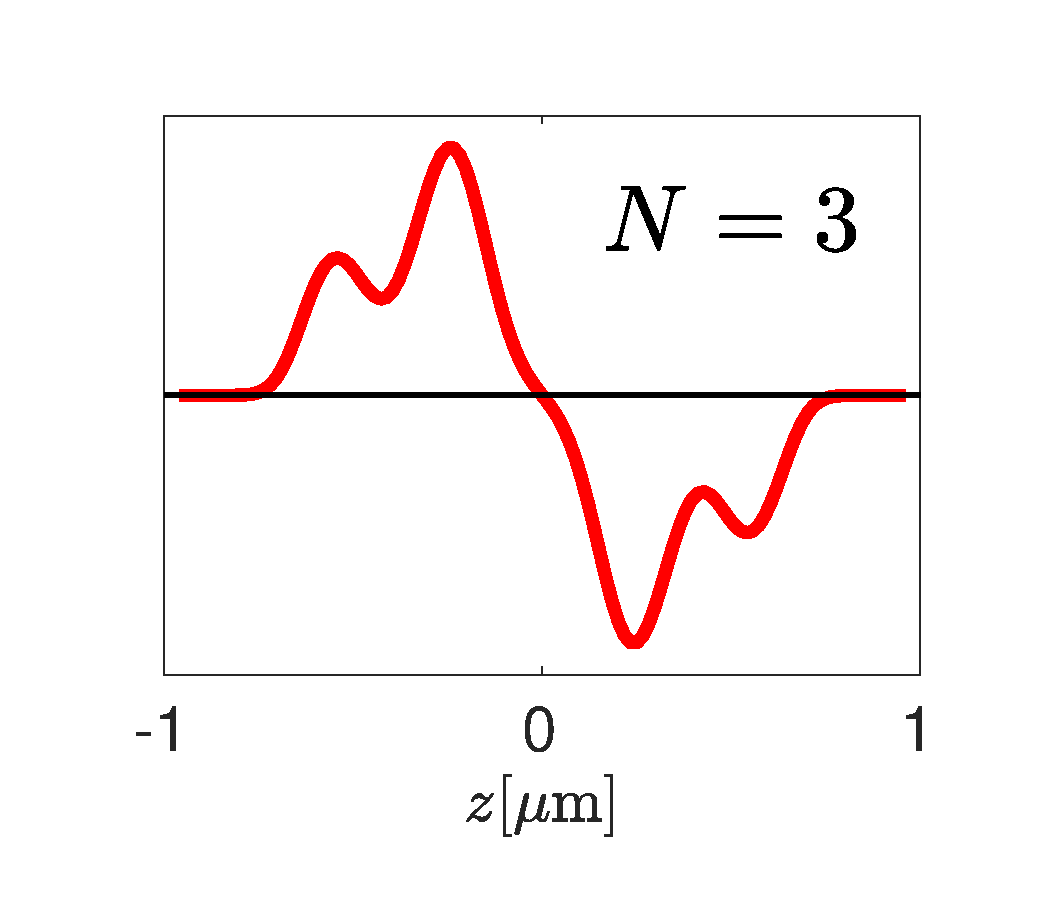
\includegraphics[width=0.49\columnwidth]{Fig_WaveFunction_difference_3_part.pdf}
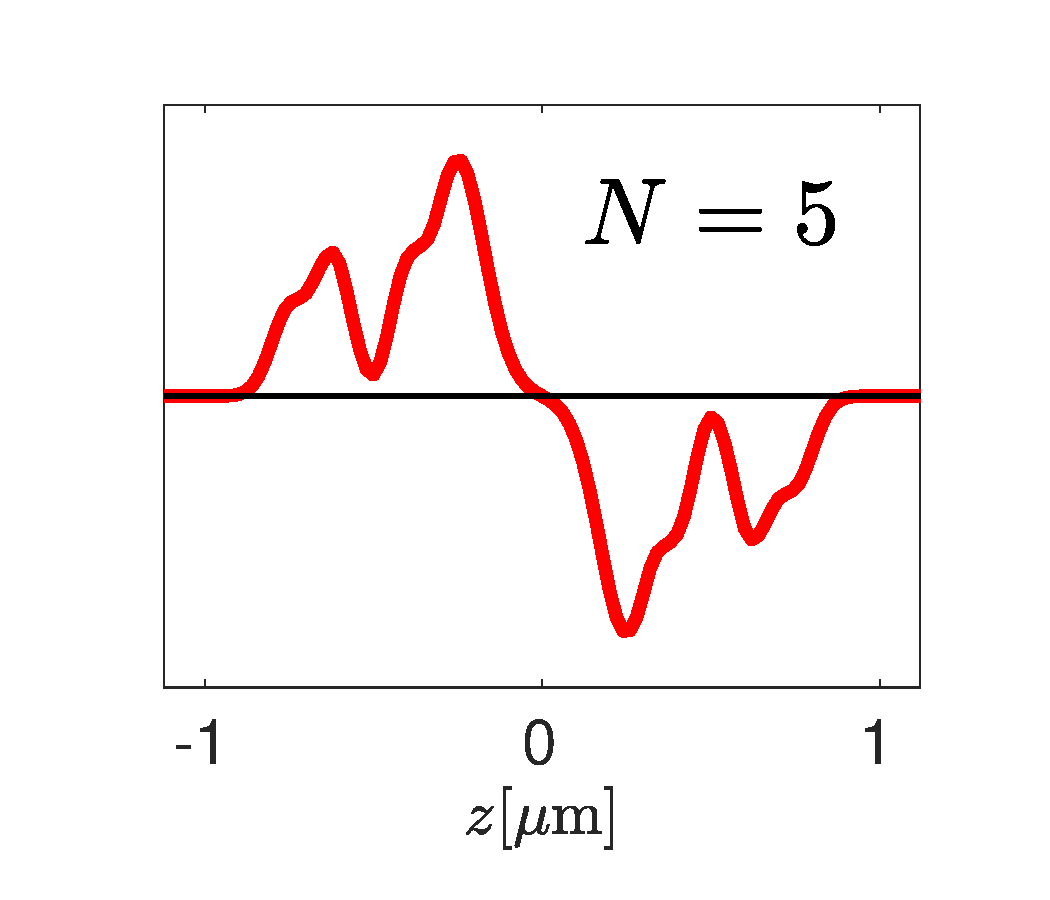
\includegraphics[width=0.49\columnwidth]{Fig_WaveFunction_difference_N_5.pdf}
 \caption{
 \label{fig:charge_conrast}
Smeared  charge density difference, $\Delta \rho(z)$, between the left and right polarized states 
 for $N=3$ and $N=5$ as a function of the bias, $\epsilon$. The peaks emerging on the sides indicates, that during the tunneling all the three particles change their positions. }
\end{center}
\end{figure}

 
 We present  $\rho(\chi)$  for $N=3$ particles in Fig.~\ref{fig:charge_distribution}
for a set of parameters $\alpha$. The classical ground state  becomes twofold degenerate at  
$\alpha=\alpha^{N=3}_\text{cl}\approx 4.45$. Quantum fluctuations, however, shift this threshold
to $\alpha^{N=3}_\text{0}\approx 6.9$, and tunneling takes place only for  $\alpha \gtrsim  6.3$. 
Fig.~\ref{fig:charge_distribution} also displays the charge polarization, Eq.~\eqref{eq:pol}. 
The main contribution to  the polarization comes from the tunneling of the central electron, 
and the rearrangement of  electrons on the right and the left yields a much smaller contribution. 
At $\epsilon\approx 0$, the central electron is strongly delocalized between the two sides, while the 
lateral electrons gradually shift as the central charge is transferred. 





\begin{figure*}[t!]
    \begin{center}
     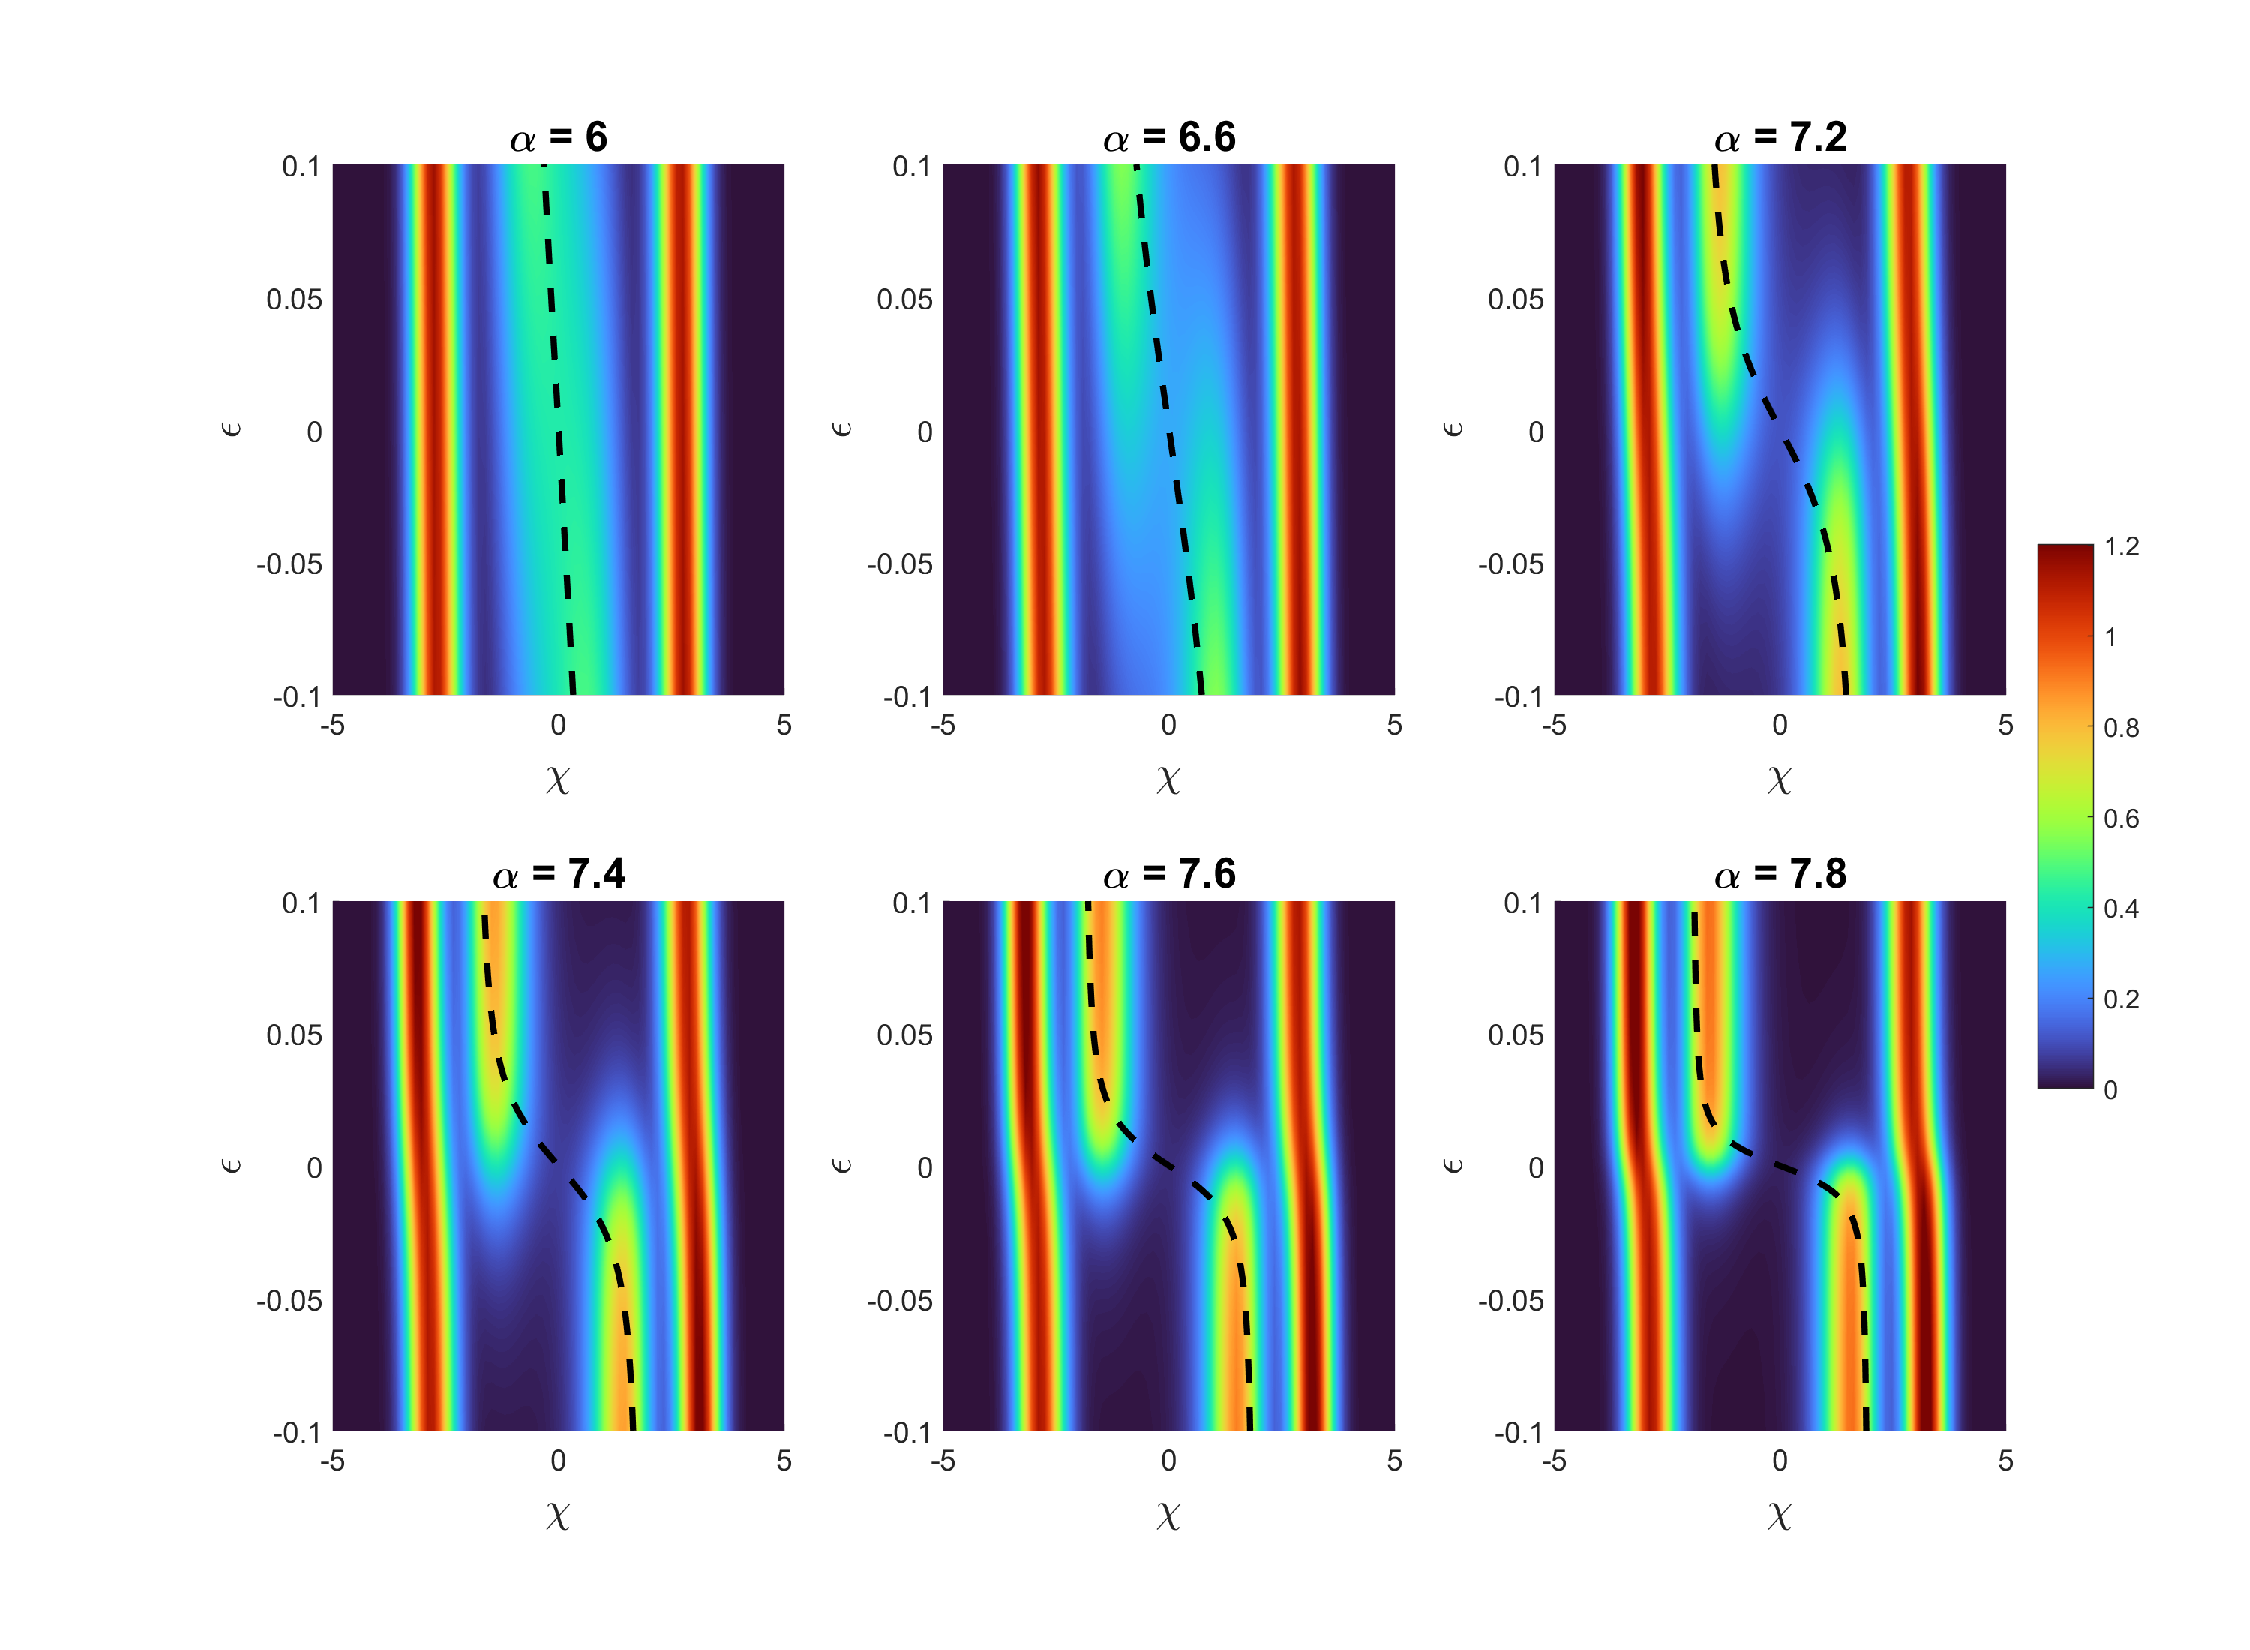
\includegraphics[width=1.6\columnwidth]{SupMatFig_DensitySeries}
     \caption{
      \label{fig:charge_distribution}
     Charge distribution (color code) and the polarization (dashed line)  for $N = 3$ particles. The classical critical point is at $\alpha_\text{cl}^{N=3} \approx 4.45$, but tunneling occurs only above $\alpha^{N=3}_0 \approx 6.9$. Most of the polarization is carried by the central electron. Quantum fluctuations of lateral electrons facilitate the tunneling process.}
  \end{center}
     \end{figure*}

This seems to suggest that lateral electrons are merely spectators of the tunneling event. 
This is, however, not true. As already discussed above, the profile $\Delta \rho$ clearly demonstrates that 
\emph{all electrons} participate in the tunneling process. This is corroborated 
by our instanton computations, which show that lateral electrons participate in 
collective vibrations and thereby  enhance quantum fluctuations,  
which largely facilitate the quantum-tunneling process, as captured by the 
increased prefactor $R_0$ in Eq.~\eqref{eq:instanton}.

% \begin{figure}[h!]
% 	\begin{center}
% 		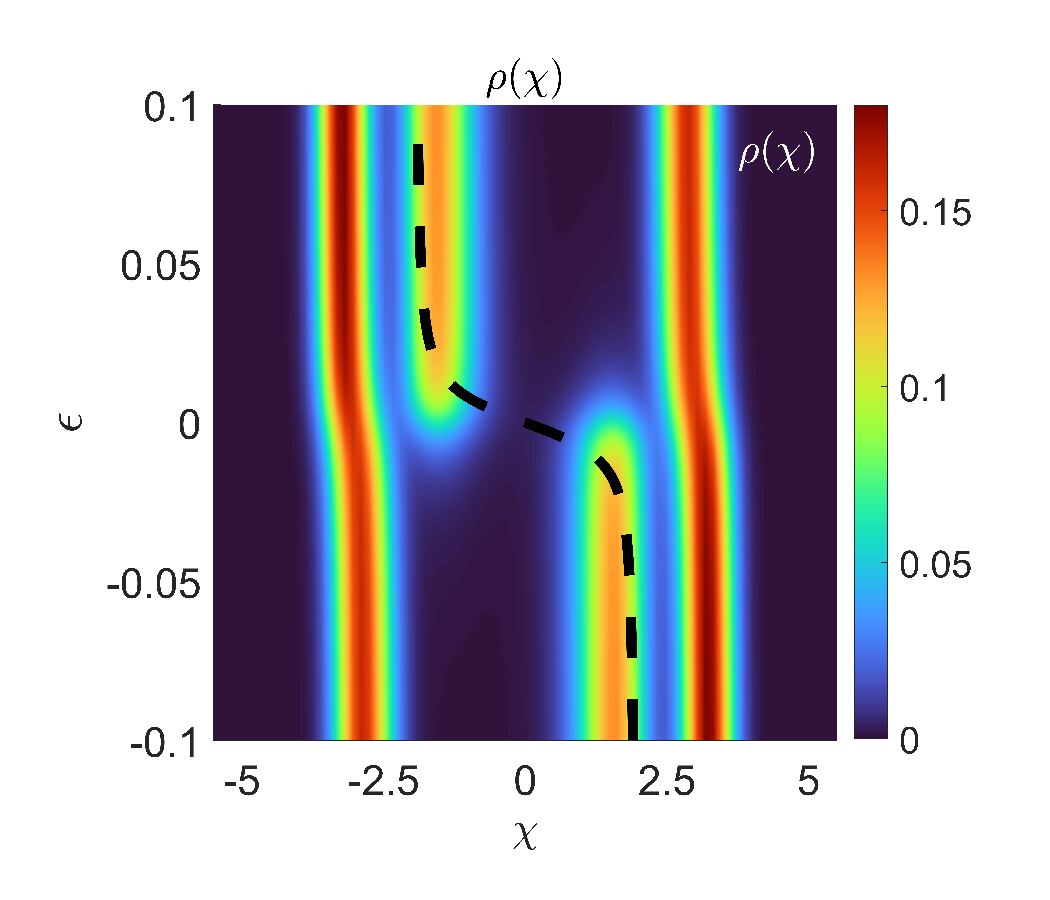
\includegraphics[width=1\columnwidth]{Fig_Polarization_2D}
		
% 		\caption{Top: Charge density as a function of the dimensionless electric field $\epsilon$ at $\alpha = 7.8$ and $\eta = 20$. The dashed line denotes the polarization in the system.}
% 	\end{center}
% \end{figure}

	
\section{Conclusion}\label{sec:conclusions}
In this work, we combined several theoretical approaches to describe the tunneling of 
a small Wigner crystal  confined within a suspended carbon nanotube and subject to a 
double-well potential, studied experimentally in Ref.~\cite{Shapir.2019}.  For an odd number of electrons
and for sufficiently high barriers,
 the classical ground state of the crystal becomes  degenerate,  and the crystal tunnels between these two states. 

A combination of instanton theory, Density Matrix Renormalization Group 
and  a peculiar Exact Diagonalization method allowed us to describe the low energy spectrum of the crystal
as well as its charge distribution,  and determine the amplitude of collective tunneling in this very strongly interacting regime, and compare  with the experimental results~\cite{Shapir.2019}.
The methods above provide us  a consistent picture,    compare well with the experiments, and
 provide a quantitative theory for the experimental data in Ref.~\cite{Shapir.2019}.


Interestingly, the tunneling crossover does not take place at the classical bifurcation point, as naively expected, 
but due to quantum fluctuations it is shifted towards somewhat 
higher barrier values (higher values of $\alpha$ in Eq.~\eqref{eq:Hamiltonian_2}). 
Indeed, our calculations clearly demonstrate both the importance of quantum fluctuations 
and the collective nature of tunneling. 


Rather surprisingly, we find that the presence of other 
particles \emph{increases} the tunneling amplitude rather than 
reducing it.  
Indeed, in typical tunneling problems the presence of environment leads to a 
\emph{suppression} of tunneling due to Anderson's orthogonality catastrophe \cite{Anderson1967,Leggett1987}.
The physics behind this latter phenomenon is that the motion of one (test) particle influences the 
wave function of all other particles, too, which therefore act back and suppress the motion of 
aforementioned particle. In our case, however,  collective quantum fluctuations of the electron 
chain seem to play a much more important  role: they facilitate the  motion of the innermost electron, 
which is mostly responsible for the tunneling.  This effect is very similar to 
the one found in the case of infinitely long one-dimensional chains, where quantum fluctuations can strongly 
\emph{suppress} the  strength of a pinning center, even in the limit of very strong interactions, 
$r_s \gg 1$, where  pinning  is a strongly relevant perturbation~\cite{Shklovskii.1992,KaneFisher1992}.

Quite astonishingly, the experimental data as well as  our theoretical curves   exhibit a universal 
scaling collapse.  At a first sight, this seems quite natural: one can identify a single collective coordinate 
within the instanton theory, which moves in an effective double well potential, 
and is responsible for the tunneling of the crystal. This would support the emergence of
a universal tunneling curve – apart from some overall scaling factors. However,  the remaining 
degrees of freedom  renormalize the tunneling amplitude for $N\ge 3$ particles
by a renormalization factor that has an intrinsic gate voltage dependence.  Apparently, the latter 
renormalization factor, although without an obvious reason,  does not spoil the 
aforementioned universal scaling within  our computational accuracy. 


Finally, let us  briefly commenting  on  the role of 
spin and chiral degrees of freedom. Electrons or holes in a nanotube 
 possess chirality and spin quantum numbers. 
In this work, however, we assumed that the spin sector is completely incoherent, and can therefore be 
considered as classical. This is certainly justified for the experiments in Ref.~\cite{Shapir.2019}. 
At very low temperatures or smaller interactions, however,  exchange processes 
may become important, and disregarding the spin sector entirely may not  be  quite appropriate~\cite{FieteBalents2004,Fiete2007}. 
This is further complicated by the presence of spin-orbit coupling, which couples spin 
and chiral degrees of freedom, and leads to the freezing out of the charge carriers' SU(4) spin.  
The description of the residual SU(2) degrees  of freedom~\cite{Sarkany.2017}  and their impact 
on the tunneling process at low temperatures  as well as the role of the  SU(4)$\to$SU(2) cross-over 
is an open and challenging problem, left for future investigation. 

% \appendix
% \section{???}
\acknowledgments
This research is supported by the National Research, Development and Innovation Office NKFIH through research grants 
Nos. K134983, and  %Legeza dinamika
% K138606, %Kormos
K132146,  % Pályi	topolóia
and within the Quantum Information National Laboratory of Hungary (Grant No. 2022-2.1.1-NL-2022-00004). 
%(Project No. 2017-1.2.1-NKP-2017-00001). 
%
M.A.W. has also been supported by the Janos Bolyai Research Scholarship of the
Hungarian Academy of Sciences and by the ÚNKP-22-5-BME-330 New National Excellence Program of the Ministry for Culture and Innovation from the source of the National Research, Development and Innovation Fund
%
C.P.M acknowledges support by the Ministry of Research, Innovation and Digitization, CNCS/CCCDI–UEFISCDI, 
under projects number PN-III-P4-ID-PCE-2020-0277 and the project for funding the excellence, contract 
No. 29 PFE/30.12.2021. 
O.L. has been supported by
Scalable and Predictive methods for Excitation and Correlated phenomena 
(SPEC), funded as part of the Computational Chemical Sciences Program by 
the U.S. Department of Energy (DOE), Office of Science, Office of Basic 
Energy Sciences, Division of Chemical Sciences, Geosciences, and 
Biosciences at Pacific Northwest National Laboratory.
%
D.S. acknowledges the professional support of the doctoral student scholarship program of the co-operative doctoral program of the Ministry for Innovation and Technology from the source of the National Research, Development and Innovation fund.
%
\appendix

\section{Computation of the instanton prefactor.}\label{app:prefactor}
Performing the Gaussian integral in Eq.~\eqref{eq:K_full}, one finds \cite{Milnikov.2001}
\begin{gather}
K(\mathbold{\chi}_0^\prime, \mathbold{\chi}_0) = \e^{-S_E} \sqrt{ \frac{2S_E}{\pi}} \left[ \frac{\det^\prime \left(-\partial_\vartheta^2 + V^{\prime \prime}_0 (\vartheta))   \right)}{\det\left(-\partial_\vartheta^2 + 
\omega^2_{\rm{soft}}   \right)}  \right]^{-1/2} \label{eq:K_sep} \\
\times\left[  \frac{\det^\prime \left(-\partial_\vartheta^2 {\bf{1}} + {\bf{\Omega}}^2 (\vartheta)   \right)}{\det\left(-\partial_\vartheta^2 {\bf{1}}+ {\bf{\Omega}}^2_0   \right)}   \right]^{-1/2}.\nonumber
\end{gather}
Here the first line represents the propagator's classical contribution, whereas the second line 
denotes the contribution arising from quantum fluctuations.

The softest vibrational mode at the base of the classical trajectory  $\bchi_{cl}(\tau)$ has a frequency  $\omega_{\rm{soft}}$, and $\det^\prime$ denotes the functional determinant, computed  by excluding the zero eigenvalue in the energy spectrum of the tunneling.

The  $(\n-1) \times (\n-1)$ matrix   ${\bf{\Omega}}_0$ represents the eigenfrequencies around the equilibrium position, $\bchi_0$. The $(\n-1)\times (\n -1)$ matrix ${\bf{\Omega}}(\vartheta)$ is computed using the vibrational eigenvectors along the instanton trajectory. Technically, to compute the contribution coming from the quantum fluctuations is a delicate issue. We followed the approach introduced in Ref.~\cite{Milnikov.2001} and  introduce the Jacobian fields through $\left(-\partial_\vartheta^2 {\bf{1}} + {\bf{\Omega}}^2 (\vartheta)   \right) \bJ(\vartheta)=0$ which is related with the derivative of the instanton $\bkappa(\vartheta) \propto \dot \bchi(\vartheta) $. Introducing a function ${\bf \Xi} (\vartheta) = \dot \bkappa(\vartheta)\, \bkappa(\vartheta)^{-1}$ that satisfies a differential equation,  ${\bf{\dot{\Xi}}} = \varrho /(1 - \vartheta^2)\left({\bf{\Omega}^2}(\vartheta) - {\bf{\Xi}}^2(\vartheta)\right)$, with the boundary condition that the particles behavior is of a harmonic oscillator, we can express the tunnel splitting in a compact form.

An essential aspect of this calculation is the introduction of a coordinate basis transformation on the $\n$ dimensional trajectory. The new basis consists of one parallel and $\n-1$ perpendicular unit vectors with respect to the trajectory, as opposed to $\n$ coordinates that describe the independent particles. It is found that the trajectory's direction is parallel to the eigenvector of the softest vibrational eigenmode.

In this description the trajectory and subsequent calculations can be simplified to an arc-length parametrized effectively one-dimensional description. This takes place in the effective potential, that is created by the collective motion of particles as in Fig. \ref{fig:traj}. This enables us to calculate the quantity $P[{\mathbold{\chi}}_{cl}(s)] $ as a one-dimensional equation. This renormalization constant depends on the momentum-like quantity $p_0 = \sqrt{2 [v_{\n}^{\rm{max}} - v_{\n}^{\rm{min}}]}$
\begin{equation}
% P[{\mathbold{\chi}}_{cl}]
P[{\mathbold{\chi}}_{cl}(s)] = \exp\left\lbrace \int\limits_{-1}^0 {\rm{d}}\vartheta\, \frac{\varrho}{(1 - \vartheta^2)} \left( \omega_{\rm{soft}} - \frac{\partial p_0(s)}{\partial s} \right) \right\rbrace.
\end{equation}

 This arc-length parametrized picture makes it possible to express $\mathbold{\Omega}$ by the curvature of the trajectory parametrized either by imaginary time or arc-length, although the two descriptions yield the same results. Solving numerically the set of differential equations ${\bf{\dot{\Xi}}} = \varrho /(1 - \vartheta^2)\left({\bf{\Omega}^2}(\vartheta) - {\bf{\Xi}}^2(\vartheta)\right)$ with the appropriate boundary conditions that states, that indeed for times close to $\vartheta = \pm 1$ the particles behave like a collective harmonic oscillator.

The renormalization factor $R_0(\alpha, \n)$ then can be expressed as
\begin{gather}
	R_0(\alpha, \n) = \sqrt{\frac{\det {\bf{\Omega}}_0}{\det {\bf{\Xi}}(0)}}\times\nonumber \\ \exp \left\lbrace \int\limits_{-1}^0 {\rm{d}}\vartheta \, \frac{\varrho}{(1 - \vartheta^2)}\,{\rm{Tr}}( {\bf{\Omega}}_0 -  {\bf{\Xi}}(\vartheta))\right\rbrace.
\end{gather}


\bibliography{references}

\end{document}
 